\documentclass[platex]{jsarticle}
\usepackage[dvipdfmx]{graphicx}
\usepackage{ascmac}
\usepackage{listings}
\usepackage[color]{macros}
\usepackage{comment}
 
\setlength{\oddsidemargin}{-5mm}
\setlength{\textwidth}{160mm}
\setlength{\topmargin}{-5mm}
\setlength{\textheight}{230mm}

%%%%%%%%%%%%%%%%%%%%%%%%%%%%%%%%%%%%%%%%%%%%%%%%%%%%%%%%%%%

\title{令和 5 年度地球惑星物理学演習 \\
       UNIXその 1 \\
       --- UNIX の基礎的概念・基本コマンドとシェル ---}
\author{担当:臼井健人、宮武勇介
  %  \thanks{大気海洋科学講座 \href{https://www-aos.eps.s.u-tokyo.ac.jp/~miura/}{三浦研究室} M1,
  %  \mail{khashimoto@eps.s.u-tokyo.ac.jp}}
  \\ \\
   テキスト: 堀田 (2004, 2005) \\
   改訂: 吉武 (2006)、太田, 吉武 (2007)、渡邊 (2009)、\\ 横田 (2010)、小寺 (2011)、仲谷 (2012)、\\
   山上 (2013)、伊藤 (2014)、南原 (2015)、\\ 宮寺 (2016)、植村 (2017)、鈴木 (2018)、\\
   \UTF{9AD9}木(2019)、湯本(2020)、坂井(2021)、\\
   橋本(2022)、臼井、宮武(2023)}
\date{実施日: 2023/4/6} %\qquad 最終更新: \ProcessDateTime}

% 01-shell.tex        02-unix-linux.tex       03-cui-gui.tex
% 04-commands.tex     05-man-command.tex      06-shell-le.tex
% 07-file-system.tex  08-file-manip.tex       09-user-group.tex
% 10-process.tex      11-pipe-redirect.tex    12-shell-itself.tex
% 13-printing.tex     14-removable-media.tex  15-kadai.tex
% \includeonly{10-process,11-pipe-redirect}

\setcounter{tocdepth}{1}

%%%%%%%%%%%%%%%%%%%%%%%%%%%%%%%%%%%%%%%%%%%%%%%%%%%%%%%%%%%%
\begin{document}
\maketitle

\vfill


\begin{center}
  
\includegraphics[width=.24\textwidth]{./images/penguin.eps}
  
\includegraphics[width=.24\textwidth]{./images/penguin.eps}
  
\includegraphics[width=.24\textwidth]{./images/penguin.eps}
  
\includegraphics[width=.24\textwidth]{./images/penguin.eps}\\
  \small
  figure:
  \textbf{Tux}, the official muscot of the Linux kernel,\\
  by \textit{Larry Ewing} <\texttt{lewing@isc.tamu.edu}>~~
  thanks to \textit{GIMP} ({http://www.gimp.org/})
\end{center}

\vfill
\clearpage

\tableofcontents

%%%%%%%%%%%%%%%%%%%%%%%%%%%%%%%%%%%%%%%%%%%%%%%%%%%%%%%%%%%%
\section{はじめに}

 今回の目標は UNIX の基礎的な概念を理解し基本的なコマンドを使えるようになるこ
 と、シェルの機能を利用して楽をする方法を知ること、UNIX について知らないことがあり
 困ったときに自力で調べて解決する方法を身に付けることです。

%%%%%%%%%%%%%%%%%%%%%%%%%%%%%%%%%%%%%%%%%%%%%%%%%%%%%%%%%%%%


\section{UNIX・Linux}

 \重要{UNIX} とは 1971 年にアメリカの電話会社 AT\&T のグラハム・ベル研究所で
 Ken Thompson と Dennis Ritchie が開発し、主に大学や研究機関で愛用され育って
 きた OS です。

 UNIX は高級言語である C 言語で書かれたために移植しやすく、現在の OS で基本と
 なる機能 (マルチユーザ / マルチプロセス周辺機器への統一的なインターフェイス、
 一貫的なファイル / 階層的ファイルシステムなど) を数多く実装したため、広く利用さ
 れることとなりました。また、ソースコードが公開されたことで UNIX をベースに独自
 の機能を追加した派生バージョンが多数出現しました。

 現在は UNIX という名前の OS があるわけではなく UNIX 系の OS を総称して UNIX
 と呼んでいます。以下でも UNIX という言葉はこの意味で使っています。この演習室
 で使っているのは \重要{Linux} という UNIX の仲間です。

 Linux は厳密には UNIX とは呼べないのですが、非常に UNIX に近い OS です。
 Linux が使えるようになれば他の UNIX を使いこなすのも容易なはずです。

 \begin{プチノート}
  Linux は日本では「リナックス」と読むのが一般的ですが、北米では「ライナックス」
  と読む人が多く、欧州では「リーヌクス」とか「リノー」とか、 Finnish (?)な読み
  方が多いそうです。
 \end{プチノート}

 Linux は、1991 年にヘルシンキ大学の学生 Linus B. Torvalds によってUNIX をモデ
 ルに開発されました。 Linus 氏は Linux のカーネルという中核部分のみを開発した
 のでカーネル部分のみを「Linux」と呼ぶのが本来は正しいのですが、現在では大抵、
 Linux カーネルで動いているシステム全体を指して「Linux」と呼んでいます。

 \subsection{GNU・Free Software Foundation・Richard Stallman 氏}
 演習室で動いている Linux のカーネルは Linus 氏が中心となって書かれたものです
 が、Linux で利用される基本コマンドやコンパイラなどはほとんど全て the GNU
 Project の製品です。

 the GNU Project とは、1985 年の春、MIT の人工知能研究所にいた Richard
 M. Stallman という人物が「ソフトウェアは ``free'' であるべき」とい
 う彼の理想を実現するために立ち上げたプロジェクトで、彼の設立した Free
 Software Foundatoin (FSF) というボランティア団体により運営されていま
 す。Richard Stallman 氏が the GNU Project において目標としたのは全て
 が ``free'' なライセンスで提供される
 \footnote{ 現在GNU ProjectはGPL(General Public License)と呼ばれるライセンスを用いていますが、このライセンスの求める``free''は必ずしも無料であることを意味しません。
 また著作権の放棄とも少し異なる概念です。
 ライセンスの条項は極めて長いですが、概ね、プログラムについて実行、改変、再配布を許可し、2次生産物に対して同じGPLライセンスを適用することを義務付けることで、
 公的に開かれたプログラム群を作ろうとする枠組みだと把握しておけばいいと思います。
 こういったライセンスはかなり色々あります。}
 、UNIX 互換のシステムを作り上げるという大変なものでした。
 Richard Stallman 氏が書いたソフトウェアには、GNU Emacs や
 コンパイラgcc\footnote{ これから Fortran の演習で使う gfortran も gcc の一部です}、
 デバッガ gdb, bison, ld, /bin/sh など、皆さんがこれからお世話になるであろう
 ソフトウェアが信じられない程沢山あります。

%%% Local Variables:
%%% mode: japanese-latex
%%% TeX-master: "01-shell"
%%% mode: auto-fill
%%% fill-column: 72
%%% End:

%%%%%%%%%%%%%%%%%%%%%%%%%%%%%%%%%%%%%%%%%%%%%%%%%%%%%%%%%%%%
%\input{03-cui-gui}


 \section{CUI と GUI}
 Microsoft Windows や macOS\footnote{ 実はmacOSもUNIXです。なので演習で習うコマンドはmacOSでも使うことができます。しかし、UNIXコマンドには系統があって、LinuxにはGNU系コマンドが入っている一方、macOSには(少し古めの)BSD系コマンドが入っています。そのためオプションなどの挙動が異なることがあり、特にawkとかgrepはかなり違っていたりします。計算機演習の講義資料はすべてGNU系コマンドを前提に作られているので、計算機演習ではmacOSではなく、DebianというLinuxのasanoという計算機を使うことにしています。}は GUI (\textbf{G}raphical \textbf{U}ser \textbf{I}nterface) と呼ばれる
 仕組みでの操作が中心となっているため、マウスでアイコンをクリックするなどの操
 作で多くのことが行えます。これに対して、UNIX ではこの GUI に加えて CUI
 (\textbf{C}ommand-line \textbf{U}ser \textbf{I}nterface あるいは
 \textbf{C}haracter \textbf{U}ser \textbf{I}nterface) という仕組みによる操作法
 も良く使われます。この CUI においては、コンピュータと主に文字のやりとりをする
 ことでさまざまな操作を行います。GUI と比較すると CUI の操作方法は敷居が高い
 ものですが、その分、慣れてしまうとGUI と比べて動作が軽快に行えるなどのさま
 ざまな利点があります。たとえば作業の自動化・再利用などは GUI ではほとんど不
 可能ですが、CUI では実にスマートに実現できます。

 逆に言えば、操作に慣れないままだと、単なる使いにくいコンピュータになってしま
 います。使い方が分かってしまうまでは不便かも知れませんが、積極的にマシンに触っ
 て、早いうちに CUI の操作になれましょう。

 CUI の操作はターミナルウィンドウとよばれるウィンドウの中で行われます。ター
 ミナルウィンドウを起動してみましょう。

 以後の作業は全てこのウィンドウの中で行います。以降、「ターミナル」とか「シェ
 ル」とかいう言葉はこれを指していると考えて下さい。
%  また、このターミナルで peep_TA & と打ち込んでリターンを押すと TA の端末画面を
%  のぞき見することができます。説明の都合で TA の画面を皆さんに見ていただきたい
%  ときがあるかも知れませんが、そのときは peep_TA を実行してみて下さい。


%%% Local Variables:
%%% mode: japanese-latex
%%% TeX-master: "01-shell"
%%% mode: auto-fill
%%% fill-column: 72
%%% End:

%%%%%%%%%%%%%%%%%%%%%%%%%%%%%%%%%%%%%%%%%%%%%%%%%%%%%%%%%%%%
%\input{04-commands}


\section{コマンド・オプション・引数}

 CUI ではコンピュータに\重要{コマンド}と呼ばれる、文字列からなる命令をターミナ
 ルに打ち込むことでさまざまな操作を行います。

 ターミナルウィンドウの中には
 \begin{terminal}~\$ \end{terminal}
 のような表示があると思います。これを\重要{プロンプト}といいます。プロンプトは
 ターミナルが入力待ちの状態であることを示すものです。ターミナルウィンドウを終
 了するときにはプロンプトにつづけて
 \begin{terminal}~\$ exit\end{terminal}
 と入力しリターンキーを押します。この操作をしないでログアウトしたりすると後に
 述べるヒストリの保存が行われなかったりと、色々不都合がありますのでログアウ
 トする前に必ず \command{exit} と入力する癖をつけるようにして下さい。

 では早速コマンドを入力してもらいたいのですが、最初に以下のコマンドを入力してください
 (自前のPC でUNIX の仮想環境を使っている人は入力しないでください)。
 \begin{terminal}~\$ ssh asano \end{terminal}
 これによって、
 演習室にあるasanoというLinuxマシンにログインします。
 初めてsshでログインする際には
 \begin{terminal}
The authenticity of host 'asano (133.11.231.4)' can't be established.
ECDSA key fingerprint is ef:e0:a3:1d:06:ba:b5:16:05:1f:aa:eb:a2:83:70:6a.
Are you sure you want to continue connecting (yes/no)? \end{terminal}
 などと尋ねられますが、気にせず
 \begin{terminal} yes \end{terminal}
 と入力しましょう。すると、以下のようにパスワード入力を求められます。
 \begin{terminal} Warning: Permanently added 'asano,133.11.231.4' (ECDSA) to the list of known hosts.
s222601@asano's password: \end{terminal}
ここでマシンのログインパスワードと同じパスワードを入力してください。
以上によってasanoにログインすることができるようになりました。
今後の演習でも、演習室のmacを使用する場合には必ず最初にssh asano を入力し、
asanoにログインするようにしましょう。
 
 それでは気を取り直して早速コマンドの練習をしていきましょう。プロンプトに続けて
 \begin{terminal}~\$ echo -e 'Hello \bs{}n World!'\end{terminal}
 と入力し、リターンキーを押して下さい。
 \begin{terminal}Hello \\ World!\end{terminal}
 のような出力が返ってきたと思います。今入力した
 \command{echo -e 'Hello \bs{}n World!'} の全体、あるいはその内の先頭の
 \command{echo} の部分をコマンドといいます。
 また、この例の場合、\term{-} (ハイフン) ではじまる \term{-e} の部分を
 \重要{オプション}、最後の \term{'Hello \bs{}n World!'} の部分を\重要
 {引数} (ひきすう、argument) と呼びます。\重要{オプション}はコマンドの動作に変
 化を加える目的で使われ、\重要{引数}はコマンドの動作の対象 (文字列とか、ファイ
 ル、ユーザとか) を指定するのに使われます。
 
 \begin{プチノート}
  シェルはユーザからの入力を受けると、スペースで区切って (tokenize して) コマ
  ンドに渡します。従ってスペースはただの区切りの意味しか持ちません。但し、
  「\term{'}」や「\term{"}」によって囲まれた文字列は 1 つの \mbox{``単語''}
  (token) としてコマンドに渡されます。その際、両側の「\term{'}」や
  「\term{"}」は取り除かれます。
  \vspace{1ex}

  このように「\term{\vs';[]\bs!\#\$\^\&\*()"<>\?|\~\`}」%
  ({\vs} は半角スペース) の各文字および改行はシェル (正確には bash; シェルや設定によって
  このような文字は異なる) にとって特別な意味を持っているので、これらをただの文字
  として認識させるにはその文字の前に「\term{\bs}」を置くことで
  \重要{エスケープ}する必要があります。
  \vspace{1ex}

  また、「\term{'}」や「\term{"}」で囲んでも同様にエスケープすることがで
  きますが、「\term{'$\cdots$'}」の中で「\term{'}」を含むことは (bash で
  は) できません。さらに「\term{"$\cdots$"}」の中で「\term{"}」と
  「\term{\$}」を使う場合にもやはり「\term{\bs}」を前置する必要があります。
 \end{プチノート}

 英語の命令文は例えば Hold me tight. のように、先頭に動詞 (hold), 続けて目的語
 (me) や副詞 (tight), という形をしていますが、オプションは副詞に、引数は目的語
 に相当していると思うとよいでしょう。

 以上まとめると、UNIX のコマンドは 1 つのコマンド、0 個以上のオプション、0 個
 以上の引数、をそれぞれ 1 つ以上のスペースで区切ったもの、という形をしています。
 最後にリターンキーを押せばコマンドが実行されます。

  \subsection*{練習課題}
 先ほどの\command{echo -e 'Hello \bs{}n World!'} のオプションを\command{-n}にしたり無しにしてみましょう。
 また、エスケープシーケンスを\command{\textbackslash n}から
 \command{\textbackslash c}や\command{\textbackslash v}に変えてみましょう。
 結果を見てこれらのオプションやエスケープシーケンスの意味を考えて下さい。
 ターミナルに\command{man echo}と入力すると、答えが分かります。

%%% Local Variables:
%%% mode: japanese-latex
%%% TeX-master: "01-shell"
%%% mode: auto-fill
%%% fill-column: 72
%%% End:

%%%%%%%%%%%%%%%%%%%%%%%%%%%%%%%%%%%%%%%%%%%%%%%%%%%%%%%%%%%%
%\input{05-man-command}


\section{man コマンド}

 \command{man} コマンドは UNIX を使えるようになる上で非常に重宝するものです。

 \command{man} は manual の略で、その名の通り各種コマンドのマニュアルを表示
 するコマンドです。例えば
 \begin{terminal}~\$ man echo\end{terminal}
 と入力してリターンを押せば \command{echo} のマニュアルが表示さ
 れます。マニュアルは \command{less} というプログラムによって表示され
 \footnote{ 正確には、環境によって異っており、\command{less} とは限りませ
 ん。}、
 スペースを押せば次のページにスクロールします。 \command{less} から抜けるには
 q キーを押します。\command{less} 画面の中で / (スラッシュ) をタイプし、続けて
 文字列を入力してリターンを押すとその文字列を検索することもできます。 n キーを
 押せば次の、Shift+n キーを押せば前の検索候補が表示されます。

 コマンド名は分からないが知りたいキーワードがある、という場合には
 \term{-k} オプションをつけて
 \begin{terminal}~\$ man -k \argument{Shiritai-Keyword}\end{terminal}
 と入力すれば\argument{Shiritai-Keyword}に関係したコマンドの一覧が表示されます。たくさ
 ん表示されすぎて画面に表示しきれない場合は後に述べるパイプの機能を利用して
 \begin{terminal}~\$ man -k \argument{Shiritai-Keyword} | less\end{terminal}
 と入力して下さい。q キーを押せば抜けることができます。何か分からないことが
 あったらすぐに \command{man} でマニュアルを読む、という癖をつけて下さい。
 他にも\command{ echo} -{-help}, \command{ info echo} という方法もあります。

%%% Local Variables:
%%% mode: japanese-latex
%%% TeX-master: "01-shell"
%%% mode: auto-fill
%%% fill-column: 72
%%% End:


%%%%%%%%%%%%%%%%%%%%%%%%%%%%%%%%%%%%%%%%%%%%%%%%%%%%%%%%%%%%
%\input{06-shell-le}

\section{ヒストリ機能・補完機能・コマンドライン編集機能}

 \subsection{ヒストリ機能}
 コマンドに複雑なオプションやたくさんの引数をつけることで入力する文字数はどんどん
 多くなっていきます。そんな中でもう一度同じコマンドを入力したい、一部分変更して
 入力したい場合にもう一度はじめから入力するのは大変です。

 そんなときは Ctrl+p\footnote{pはprevious、nはnextの頭文字です。} を
 タイプしてみましょう。すると一つ前に入力したコマンドが表示されます。さらに Ctrl+pを
 タイプすることで、どんどん過去にさかのぼってコマンドの履歴をたどることができます
 (上下カーソルキーでもコマンドの履歴を遡ることができます)。
 逆に Ctrl+n をタイプすると、今度はコマンドの履歴を古いほうから新しい方に
 たどって表示させることができます。
 これを使うと入力が圧倒的に速くなるので積極的に使っていきましょう。


 \subsection{補完機能}
 例えば文字数の長いコマンドを入力する場合、またコマンド名をきちんと覚えていな
 い場合、どのようにコマンドを入力したらよいでしょうか。ここでは Tab キーを利用
 します。ある程度までコマンドを入力した状態で Tab キーをタイプすると、全てのコ
 マンドの中から、入力した部分を先頭の文字列にとるコマンドをリストアップしてく
 れます。つまりユーザが入力したいコマンドを予測してくれるわけです。例えばコマ
 ンドラインに「\term{ech}」とだけ入力した状態で Tab キーをタイプしてみましょ
 う。\command{echo} と補完されたと思います。
 
 ちなみに「\term{e}」とだけ入力した状態でTabキーを押しても何も補完されません。
 これは他にもeから始まるコマンドが存在するためです。
 このような場合にはTabをもう一度押すとeから始まるコマンド全てが表示されます。

 Tab キーはコマンドだけでなく、ディスク内にあるディレクトリやファイル名も予測
 してくれます。コマンドの引数としてファイル名を入力することが多くあります。そ
 の際にこの Tab 補完機能は非常に役に立ちます。

 Tab キーを押しまくる癖を付けておけばかなりキータッチの回数を減らせます。タイピングミスや
 腱鞘炎の防止にもなりますので Tab キーを押しまくる癖を是非身に付けて下さい。

 \begin{プチノート}
  実は、ファイル・ディレクトリ名以外の引数やオプションも Tab キーで補完させる
  ように設定することが可能です。その設定を自分で書くこともできますが、通常は用
  意されているものを使うのが簡単です。
  \vspace{1ex}

  bash の場合は、 \path{~/.bashrc} に
  \begin{file}%
if [ -r /etc/bash_completion ]; then
  source /etc/bash_completion
fi\end{file}
  などと記述して bash を立ち上げなおして下さい。例えば
  ``\command{ls --h}'' と打ち込んだ状態で Tab キーを 2 回押すと
  \term{--h} で始まるオプションが表示されると思います。また、
  ``\command{ssh\vs}'' (\vs はスペース) と入力した状態で Tab キーを 2 回押
  すとホスト名が、``\command{cd\vs}'' の後で Tab キーを押すとディレクトリだけ
  が補完されるでしょう。
  \vspace{1ex}

  zsh や tcsh の場合にはさらに高機能な補完のシステムがあり、ユーザの作業効率
  を高めてくれます。
 \end{プチノート}

 \subsection{コマンドライン編集機能}
 GNU readline というライブラリの機能により、Emacs でのカーソル操作
 と同様のキーバインドでカーソルを動かしたりすることができます。たとえば Ctrl+a と
 打つとコマンドラインの先頭にカーソルを動かすことができますし、Ctrl+e と打つとコ
 マンドラインの最後部にカーソルを動かすことができます。また Ctrl+w と打つと現在の
 カーソル位置から直前の空白までが、 Ctrl+k と打つとカーソル位置から行末までが切り
 とられ、 Ctrl+y で直前に切り取られた文字列をペーストできます。\footnote{ ちなみにMacの一部のGUIプログラムでもこの操作は可能です。}


%%% Local Variables:
%%% mode: japanese-latex
%%% TeX-master: "01-shell"
%%% mode: auto-fill
%%% fill-column: 72
%%% End:


%%%%%%%%%%%%%%%%%%%%%%%%%%%%%%%%%%%%%%%%%%%%%%%%%%%%%%%%%%%%
%\input{07-file-system}


\section{ファイルシステム}

%%%%%%
%%%%%
%%%
%%
\begin{comment}
%%
%%%
%%%%%
%%%%%%
 \subsection{パーティション}
 ハードディスクには、物理的には一つのドライブを、論理的に複数の領域
 (\重要{パーティション}) に分割して使用する機能が用意されています。
 分割できる個数や容量はマザーボードの BIOS\footnote{ コンピュータに接続された
   ディスク、キーボード、ビデオカードなどの周辺機器を制御するプログラム群。
   通常マザーボードや拡張カード上のROM に書き込まれいるが、最近のパソコンで
   は更新することが可能となっている。} などにより異なっています。

 多くの UNIX のシステムでは (Windows 等でも)
 この機能を利用して一台のハードディスクを複数の領域に区切って、あたかも複数台
 のハードディスクがあるかのように利用しています。こうして、それぞれのパーティ
 ションについて「システム用の領域」「ユーザのデータ用の領域」のように使い分け
 ておくことで、ファイル情報が消失するなどの事故が起きても、失うデータを小さく
 することができます。

 また、パーティションごとに異なる OS をインストールして、複数の OS を一台のハー
 ドディスクの中に共存させ、マシンの起動時に立ち上げる OS を選択する、という使
 い方もあります。(いわゆるデュアルブートなど。)


%%%%%%
%%%%%
%%%
%%
\end{comment}
%%
%%%
%%%%%
%%%%%%

 \subsection{ファイルとディレクトリ}
 UNIX や Windows, Mac OS などほとんどの OS は様々なデータを整理するのに、\重要
 {ファイル}と\重要{ディレクトリ} (フォルダ) という構造を採用しています。文書や
 画像などの一連のデータはファイルと呼ばれていて、現実の世界ではルーズリーフに
 例えるとわかりやすいでしょうか。コンピュータを使い込んでいくと、すぐに大量の
 ファイルがたまっていき収拾がつかなくなってしまいます。これらを整理するための
 入れ物がディレクトリです。ルーズリーフを束ねるバインダですね。たくさんのファ
 イルを作っていくと、当然ディレクトリも大量に作られて、整理が必要になりますが、
 その場合は、これらのディレクトリ (子ディレクトリ) をまとめるためにさらにディ
 レクトリ (親ディレクトリ)を作ります。このディレクトリはバインダをためる本棚に
 相当します。このように、ディレクトリはいくつでも入れ子状にすることができます。
 以上のように、ファイルとディレクトリの構造をとることによって、データを効率よ
 く整理することができます。
 
 \subsubsection{ファイルの名前}
 全てのファイルには名前が付いています。自分でファイルを作る場合には好きな名前を
 付けることができますが、UNIX で付けられるファイル名は、多くの場合 255バイト
  (半角英数字で 255 文字、日本語のような 1 文字が複数バイトの文字を使うと
  もっと少なくなります) までという制約があります。あまり長い名前を付けても
  不便なだけなので、分かりやすい名前を付けるのがよいでしょう。

 ファイルに名前を付けるときには大文字と小文字の英数字、そしていくつかの記号を
 使うことができます。大文字と小文字は区別されます。

 ターミナルでファイルを操作する可能性があるなら、記号はできれば英数字、
 ハイフン (\path{-}), ピリオド(\path{.}), アンダースコア (\path{_}) だけ
 を使うようにした方がよいでしょう。
 他の多くの記号はターミナルでコマンドを入力する際に特別な意味を持つため、
 ターミナルでファイル名のつもりで入力すると、コマンドが意図しない動作を起こしたりします。
 (第5節で書いたようにエスケープ記号を前に置けばただの文字として使うことはできますが、やめましょう)。
 ファイル名の先頭と末尾に記号を使うのも一般に控えたほうが良いとされます。\footnote{ 例えば、ハイフン(\path{-})を
 名前の最初につけるとコマンドの引数のつもりで入力してもオプションとして扱われてしまいます。}。
   また、日本語の入ったファイル名を付けるのも避けた方が
 よいです。面倒なようですが、どのような場面でもリスクのない
 命名規則を使うよう心がけるべきです。
 \footnote{ \path{https://xkcd.com/327/}}

 \subsubsection{拡張子}
 ピリオド (\path{.}) はファイルの種類を明示したいときに使われることがあります。
 たとえば \path{index.html} という名前のファイルは、最後のピリオド以下の部分
 「\path{.html}」によって HTML 形式のファイルであることが明示されています。こ
 れをファイルの\重要{拡張子}と呼びます。

 \subsubsection{隠しファイル (ドットファイル)}
 まず、ターミナルに \command{ls /tmp/} と入力してみて下さい。何も表示されませんね。
 では、次にターミナルに \command{ls -a /tmp/} と入力してみて下さい。
 今度はピリオド (\path{.}) で始まるファイルがいくつか表示されたと思います。
 
 このように、名前がピリオドで始まるファイルはいわゆる隠しファイルとなっており、
 通常 \command{ls} コマンドなどでは表示されません。主にアプリケーションの
 ユーザごとの設定ファイルなど、誤って消去しては困るようなファイルが
 隠しファイルになっています (e.g., \path{.emacs})。
 隠しファイルを見るには \command{ls -a} とコマンドを入力する必要があります。


 \subsection{特別な意味・呼び名のあるディレクトリ}

  \subsubsection{ホームディレクトリ}
  ホームディレクトリとは 1 ユーザにつき 1 つ確保される、そのユーザ専用のディ
  レクトリのことです。ユーザは、特別な理由のない限り、自分の作成したプログラ
  ムやデータをホームディレクトリに置いておくのが慣習になっています。

  自分のホームディレクトリを示すのにチルダ (\path{~}) という記号を使うことができます。
  皆さんの場合、\path{~} と\path{/home1/s2226??/} は同じディレクトリを意味します。

  また、ユーザ X のホームディレクトリを示すのに \path{~X} という記号を使うことができます。 
  例えばユーザ sakai のホームディレクトリは\path{/home2/sakai/} ですが、
  \path{~sakai/} と書いても同じディレクトリを意味します。

  \subsubsection{カレントディレクトリ}
  カレントディレクトリとは現在作業しているディレクトリのことを指します。カレ
  ントディレクトリを確認するには \command{pwd} コマンド (\textbf{p}rint
  \textbf{w}orking \textbf{d}irectory の略) を使います。カレントディレクトリ
  を示すのにドット (\path{.})  という記号を使うことができます。

  \subsubsection{親ディレクトリ}
  カレントディレクトリの一つ上の階層のディレクトリを親ディレクトリといいます。
  親ディレクトリを示すのに \path{..} という記号を使うことができます。例えば
  カレントディレクトリが \path{/home2/s222600/matrix/revolutions/} の場合を考
  えると \path{../../harry_potter/prisoner_Azkaban/} は
  \path{/home2/s222600/harry_potter/prisoner_Azkaban/} と同じです。

  \subsubsection{相対パス・絶対パス}
  ディレクトリ名には 2 通りの指定方法があります。それは\重要{相対パス}指定と
  \重要{絶対パス}指定です。相対パス指定というのは、今自分がいるディレクトリか
  ら見たときの相対的なディレクトリの名前です。絶対パス指定というのは、そのファ
  イルの本来の名前で指定することです。ファイルの本来の名前は、\mbox{`\path{/}'}
  (ルートと読みます。) という一番大きな部屋 (その中に、全てのファイルやディレ
  クトリが含まれている) から見た時の名前です。例えばさっきの例を使うとカレント
  ディレクトリが \path{/home2/s222600/matrix/revolution/} の場合
  \path{../../harry_potter/sorcerers_stone/} は相対パス指定、
  \path{/home2/s222600/harry_potter/sorcerers_stone/} は絶対パス指定です。

  \subsection*{練習課題}
 まず、カレントディレクトリを確認してみましょう。
 
 続いて\command{cd}を用いて様々なディレクトリに移動し、
 \command{pwd}でどこにいるのかを確認してみましょう。
 \command{cd}は別のディレクトリを移動するコマンド (Change Direcrory) で、
 "\command{cd} $<$ディレクトリ名$>$"のように使います
 (\command{cd ./}や \command{cd ../} とするとどこに移動するでしょう)。
 
 色々移動して遊んだら、最後に絶対パスでディレクトリ名を指定して
 最初にいたディレクトリに帰ってきましょう。おかえりなさい。

 \subsection*{練習課題}
 \重要{この後の演習に必要なので、必ず実施してください!}
 
 この演習用端末にはバグがあり、必要なディレクトリの一つが存在していません。以下のコマンドを実行して作ってやりましょう。
 \begin{terminal} ~\$ mkdir -p ~/Library/Logs/X11\end{terminal}
 さてここで、正しくディレクトリが作られたことを確認するにはどうしたら良いでしょう?



%%%%%%
%%%%%
%%%
%%
\begin{comment}
%%
%%%
%%%%%
%%%%%%

 \subsection{UNIX 的ディレクトリ構造}
 UNIX ではディレクトリの名前の付け方や利用の仕方にある慣習が存在します。これを
 知っておくと見通しがよくなり、UNIX への理解が深まるかも知れません。図
 \ref{fig:fs-tree} は UNIX の代表的なディレクトリと、そこに何が格納されている
 かを示したものです。
 \begin{figure}[h]
  \begin{center}
   \fbox{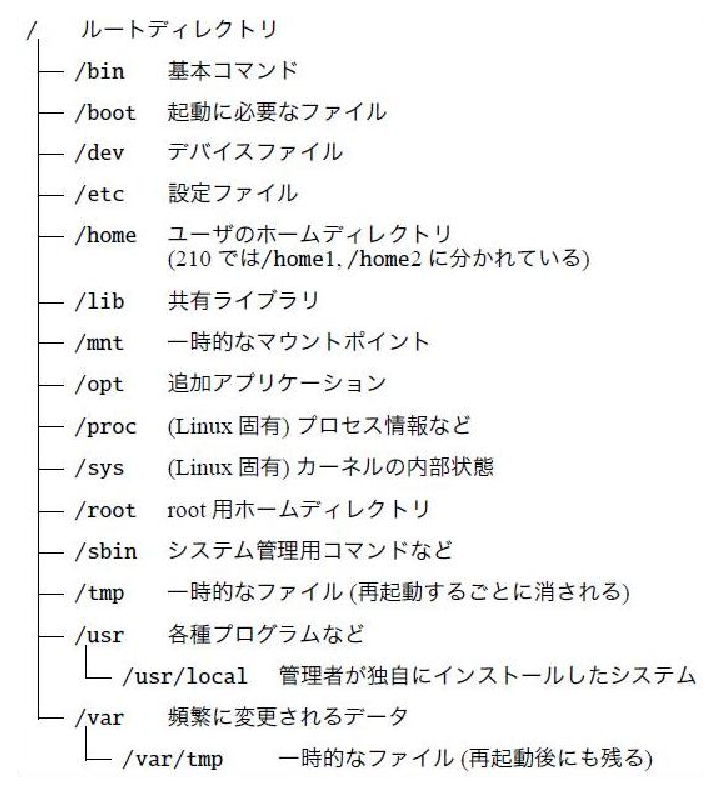
\includegraphics{images/fs-tree.eps}}
  \end{center}
  \caption{UNIX での代表的なディレクトリとその中身}
  \label{fig:fs-tree}
 \end{figure}


 \subsection{quota}
 UNIX では 1 台のマシンを複数のユーザが共有して使うことが多々あります。しかし
 ハードディスクの容量には限りがあるので、1 人のユーザが大量のデータをファイル
 に保存したりすると他のユーザがハードディスクを使えなくなってしまいます。

 それを解消するために、複数のユーザが共有するシステムでは quota と呼ばれる機
 構が働いていることがよくあります。これはユーザに対してディスクの使用量を制限
 するもので、ユーザ 1 人 1 人に対しもしくはグループ単位で、パーティション毎に
 ディスク使用量またはファイル数を制限することができます。
 \begin{description}
  \item[制限の方法]
   \begin{tabular}[t]{rl}
    \重要{block quota} & ディスクの割当を容量 (ブロック\footnotemark) で制限 \\
    \重要{inode quota} & ディスクの割当をファイル数 (inode 数) で制限 \\
                       & および、上記の組み合わせ
   \end{tabular}
   \footnotetext{ 通常は 1 block = 1 k byte = 1024 byte の単位で表示する。
     ファイルシステム上のブロックサイズとは限らない。}
  \item[\重要{ソフトリミット} (Soft Limit)] ~ \\
	     ソフトリミットとは、quota でディスクの使用量を制限されたユーザ
	     がそのパーティション上で使用可能な最大のディスク容量をいいます。
  \item[\重要{ハードリミット} (Hard Limit)] ~ \\
	     ハードリミットとは、ディスク使用量の絶対的な制限で、quota でディ
	     スクの使用量を制限されたユーザは、ハードリミットを越えることが
	     出来ません。
  \item[猶予期間 (Grace Time)] ~ \\
	     猶予期間とは、ソフトリミットが強制的に実行されるまでの期間のこ
	     とで、この期間にのみハードリミットまでディスクを使用することが
	     可能になります。通常は 1 週間程です。
 \end{description}
 つまり、ハードリミットはどうやっても超えることはできないのですが、ソフトリミッ
 トは超えられます。しかし{\gtfamily ソフトリミットを超えた状態で猶予期間を過ぎ
 るとログインができなくなります}。


  \subsubsection{quota 関連のコマンド}
  自分の quota およびディスク使用量を知るには \command{quota} コマンド
  \footnote{ 210の端末ではquotaの設定をしていないので、コマンドを入力して
  もエラーとなります。eccsの端末では設定されているそうです。}を使用
  します。
  {\setlength\narrowframewidth{4em}
    \begin{terminal}%
~\$ quota -v
Disk quotas for user s222600 (uid 50600):
     Filesystem  blocks    quota    limit   grace   files   quota   limit   grace
     sakura:/home1    6852  9000000 10000000             325       0       0
     sakura:/home2      30   100000   100000             204       0       0\end{terminal}}
  のようにします。出力の \path{sakura:/home1} $\cdots$ の行は、\path{/home1} 以
  下のファイルシステムにおいて\footnote{ sakura というのは \path{/home1} が実際に
  存在しているマシンの名前です。}、現在のディスク使用量が 6852~kB であり、ソフ
  トリミットは 9000000~kB ($\approx$ 9~GB), ハードリミットは 10000000~kB
  ($\approx$ 10~GB) であることを示しています。また、所有するファイルの総数は
  325 個で、inode quota のソフトリミット・ハードリミットは共に 0, つまり無制限
  であることを表しています。
  もしも
  {\setlength\narrowframewidth{4em}
   \begin{terminal}%
~\$ quota -v
Disk quotas for user s12345 (uid 65432):
     Filesystem  blocks    quota   limit   grace   files   quota   limit   grace
     sakura:/home1 4733286* 4000000 5000000   4days   15290       0       0\end{terminal}}
  上記のような出力が得られた場合、使用しているディスク容量がソフトリミットを
  超えており、4 日以内に対処しなければログインできなくなることが示されていま
  す。
  
  
  %%%%%%
%%%%%
%%%
%%
\end{comment}
%%
%%%
%%%%%
%%%%%%


%%% Local Variables:
%%% mode: japanese-latex
%%% TeX-master: "01-shell"
%%% mode: auto-fill
%%% fill-column: 72
%%% End:


%%%%%%%%%%%%%%%%%%%%%%%%%%%%%%%%%%%%%%%%%%%%%%%%%%%%%%%%%%%%
%\input{08-file-manip}

\section{ファイル操作}

 これまでにファイル・ディレクトリの基本的な概念、用語を学習しました。また、
 \command{man} コマンドについても学びました。そこで、今まで使ったコマンドと
 そのオプションについて \command{man} コマンドで調べてみて、
 提出課題1, 2をやってみて下さい。


%%% Local Variables:
%%% mode: japanese-latex
%%% TeX-master: "01-shell"
%%% mode: auto-fill
%%% fill-column: 72
%%% End:


%%%%%%%%%%%%%%%%%%%%%%%%%%%%%%%%%%%%%%%%%%%%%%%%%%%%%%%%%%%%
%\input{09-user-group}


\section{ユーザ・グループ}

 \subsection{スーパーユーザ}
 UNIX には \重要{スーパーユーザ} (\重要{root}) という特殊なユーザがいます。
 root ユーザはシステム管理をするためのユーザで、他のユーザのファイルを消したり、
 ユーザそのものを追加したり消去したり、アカウントを停止したり、他のユーザやシ
 ステム全体のプロセスを止めたり、とにかく何でもできるユーザです。演習室では
 admin210 という学生の管理者集団がボランティアで 演習室マシンのシステムを管理しており、
 admin210 のメンバーたちが root 権限を持っています。

 \subsection{ユーザとグループ}
 ユーザには\重要{ユーザ名}と\重要{所属グループ}という情報があります。ユーザ名
 は説明するまでもなく、自分のユーザ名です。所属グループは自分の所属するグルー
 プであって、ユーザは少くとも一つのグループに所属し、複数のグループに所属する
 こともできます。ユーザの所属するグループのうち一つは特別なグループで\重要{プ
 ライマリグループ}と呼ばれ、ファイルなどを作成した時にそのファイルの所有グルー
 プとして使われます。

 グループへの所属登録自体は管理者 (root) が行います。また、ユーザ名やグループ
 名には数値で表された識別子 (ID) が関連付けられています。\command{id} コマンド
 を使うことで自分や他のユーザの情報を見ることができます。
 \begin{terminal}~\$ id\end{terminal}
 と打ってみて下さい。
 \begin{terminal}%
uid=50600(s222600) gid=20000(student) groups=20000(student)\end{terminal}
 のような出力
 が返ってきたと思います。

 これによって得られる表示のうち uid はユーザ ID とユーザ名、gid はプライマリグ
 ループ ID とプライマリグループ名、groups は自分の所属する全グループ ID とグ
 ループ名です。

 このように、210 では学生ユーザはみな student というグループに所属しています。
 admin210 のメンバーになるとこの他 admin (gid=21000) というグループにも所属する
 ようになります。また TA や教官は ta (gid=20090) というグループに所属していま
 す。また、
 \begin{terminal}~\$ id \argument{username}\end{terminal}
 でユーザ \argument{username} の情報をみることができます。

 \subsection{ファイルの所有者}
 UNIX ではそのファイルが誰のものかを
 \begin{enumerate}
  \item[1.] owner (所有者)
  \item[2.] group (所有グループ)
  \item[3.] other (他人)
 \end{enumerate}
 の 3 つに分けて区別しています。1. はそのファイルを所有する者、2. はそのファイ
 ルを所有するグループです。3. は所有者でなく 2. のグループにも属さないユーザを
 表わします。

 自分の所有するファイルでも owner を変更することはできませんが (root にはでき
 ます)、自分の所有するファイルなら自分の所属するグループのいずれかへファイルの
 グループを変更できます。このときに利用するコマンドは \command{chgrp} です。
 \begin{terminal}%
~\$ chgrp \argument{groupname} \argument{filename}
\end{terminal}
 これでファイル \argument{filename} の所有グループが \argument{groupname} に変
 更されます。ディレクトリの中身も全て所有グループを変えたいのならば
 「\term{-R}」オプションをつけます。
 \begin{terminal}%
~\$ chgrp -R \argument{groupname} \argument{dirname}
\end{terminal}
 但し、自分の所属しないグループを所有グループにすることはできませんので
 student グループにしか所属していない皆さんは \command{chgrp} コマンドを使うこ
 とはないでしょう。

 \subsection{パーミッション}
 ファイルやディレクトリに対するアクセス許可のことを\重要{パーミッション}といい
 ます。owner/group/other に対して
 \begin{itemize}
  \item \term{r} :\quad 読み取り許可
  \item \term{w} :\quad 書き込み許可
  \item \term{x} :\quad 実行許可
 \end{itemize}
 を与えることができ、また、複数組み合わせることもできます。これらの意味すると
 ころはファイルかディレクトリかで異っており、次の表のようになります
 \begin{center}
  \begin{tabular}{|c|c|c|} \hline
   & ファイル   & ディレクトリ \\ \hline
   \term{r} & ファイルの読み込み   & ディレクトリ内のファイル一覧取得   \\ \hline
   \term{w} & ファイルへの書き込み & ディレクトリ内のファイル作成・削除 \\ \hline
   \term{x} & 実行                 & ディレクトリ内へのアクセス \\ \hline
  \end{tabular}
 \end{center}
  \vspace{-1.3zw}
  \begin{プチノート}
    ディレクトリ内へのアクセスとは、そのディレクトリをカレントディレクト
    リにする、そのディレクトリの下のファイルを参照する、ということです。
    また、ディレクトリに \term{r} が付与されていなくても \term{x} が付与
    されていれば、その中のファイルにアクセスすることがでます。 (もちろん、
    ファイルそのものに適切なパーミッション設定がされていなければなりませ
    ん。)
  \end{プチノート}
 パーミッションを確認するにはコマンド \command{ls} に \term{-l} (エル) オプ
 ションをつけて使います。
 \begin{terminal}~\$ ls -l\end{terminal}
 これで出てくる
 \begin{terminal}-rw-rw-r-- $\cdots$ (省略)\end{terminal}
 のような表示がそのファイルに設定されているパーミッションになります。

 \newbox\PermissioinImage
 \setbox\PermissioinImage=\hbox{\ifColorOutput%
   \includegraphics{images/permission.0}
 \else%
   \includegraphics{images/permission.1}
 \fi}
 \newlength\temptextwidth
 \temptextwidth=\textwidth
 \advance\temptextwidth -\wd\PermissioinImage
 \begin{wrapfigure}[1]{r}{\wd\PermissioinImage}
  \begin{center}
   \scalebox{0.9}{\box\PermissioinImage}
  \end{center}
  \caption{パーミッションの見方}
  \label{fig:permission}
 \end{wrapfigure}
 \begin{minipage}[t]{\temptextwidth}
  この 10 個のパートは
  \begin{center}
   \begin{tabular}{|l|l|} \hline
    最初の 1 文字が & {\term{d} ならディレクトリ、\term{-} ならファイル} \\ \hline
    それ以降        & 3 文字 1 セットで解釈 \\
     & \quad \begin{tabular}{rl}
	      最初の 3 文字 & 持ち主   \\
	        次の 3 文字 & グループ \\
	      最後の 3 文字 & 他人
	     \end{tabular} \\ \hline
     & そのそれぞれの意味 \\
     & \qquad \begin{tabular}{cl}
	       \term{r} & 読んで良い (read) \\
	       \term{w} & 書いて良い (write) \\
	       \term{x} & 実行して良い (excute) \\
	       \term{-} & (その場所に応じて)許可しない
	      \end{tabular} \\ \hline
   \end{tabular}
  \end{center}
  のように解釈します。パーミッションは owner/group/other ごとに
  \begin{center}
   \renewcommand{\arraystretch}{.8}
   \begin{tabular}{|c|c|c|c|l|} \hline
    許可の種類 & \term{r} & \term{w} & \term{x} & \term{-} (不許可) \\ \hline
    表す数     & 4 & 2 & 1 & 0 \\ \hline
   \end{tabular}
  \end{center}
 \end{minipage}
 \vspace{1zw}

 \noindent の 3 数の和で表されることもあります (ディレクトリであるかどうかは
 評価されません)。例えば、\term{-rw-rw-r-\mbox{}-}
 や \term{-rwx-\mbox{}-\mbox{}-r-x} はそれぞれ
 \begin{center}
  \fboxsep1.5pt
  \newlength\squash
  \setlength\squash{\baselineskip}
  \addtolength\squash{-1.5pt}
  \newcommand{\ncol}{\multicolumn{1}{c}{}}
  \renewcommand{\arraystretch}{.8}
  \fbox{%
   \begin{tabular}
    {@{\:}r@{\::~~}c@{$\>+\>$}c@{$\>+\>$}c@{$\;=\;$}|@{}c@{\,}|}
    \multicolumn{5}{l@{\;}}{
      \term{-rw-rw-r-\mbox{}-} の場合
      \hfill \raisebox{-.12zw}{\scalebox{.5}{\rotatebox{90}{\rightpointleft}}}} \\ \hline
    \ncol & \ncol & \ncol & \ncol & \ncol \\[-.8\squash] \cline{5-5}
    owner & \term{r}\,(4) & \term{w}\,(2) & 0 & \,6 \\
    group & \term{r}\,(4) & \term{w}\,(2) & 0 & \,6 \\
    other & \term{r}\,(4) &            0  & 0 & \,4 \\ \cline{5-5}
   \end{tabular}%
  }
  \qquad
  \fbox{%
   \begin{tabular}
    {@{\:}r@{\::~~}c@{$\>+\>$}c@{$\>+\>$}c@{$\;=\;$}|@{}c@{\,}|}
    \multicolumn{5}{l@{\;}}{
     \term{-rwx-\mbox{}-\mbox{}-r-x} の場合
      \hfill \raisebox{-.12zw}{\scalebox{.5}{\rotatebox{90}{\rightpointleft}}}} \\ \hline
    \ncol & \ncol & \ncol & \ncol & \ncol \\[-.8\squash] \cline{5-5}
    owner & \term{r}\,(4) & \term{w}\,(2) & \term{x}\,(1) & \,7 \\
    group &            0  &            0  &     0  & \,0 \\
    other & \term{r}\,(4) &            0  & \term{x}\,(1) & \,5 \\ \cline{5-5}
   \end{tabular}%
  }
  \global\let\ncol\relax
  \global\let\squash\relax
 \end{center}
 で 664 および 705 と表現されます。この 3 数の和で表現する方法はビット演
 算 (2 進数演算) を利用していることから、「owner に \term{r} ビットが立っ
 ている」などの言い方をすることもあります。


 \subsection{chmod}
 ファイルやディレクトリのパーミッションを変更するには \command{chmod} コマンド(change mode)を用
 います。使い方については \command{man} コマンドで調べてみましょう。

 \subsection{umask}
 umask 値はファイルやディレクトリを新規作成するときのパーミッションをいくつに
 するかという設定です。この値はファイルなら 666 の補数、ディレクトリなら 777の
 補数であらわされます。どういうことかというと、umask=022 のとき新規作成される
 ファイルは (繰り下げを許さない) 8 進数の引き算で 666 - 022 = 644 で 644 となり、
 umask=022 のとき新規作成されるディレクトリは (繰り下げを許さない) 8 進数の
 引き算で 777 - 022 = 755 で 755 となる、といった具合です。

 他のユーザに自分のファイルを見られたくないと思ったら umask 値を 044、他のユー
 ザに自分のファイルを編集されたくないと思ったら umask 値を 022、見せたくもな
 いし編集もさせたくないと思ったら 066、といった感じです。ちょっと複雑ですが、
 理解しておきましょう。

 この umask 値はデフォルトでシステム規定の値となっていますが、
 \command{umask} コマンドでその値を知ることができます。また、\command{umask}
 コマンドに設定したいumask 値を引数で与えてやれば設定をかえることもできます。
 \begin{terminal}~\$ umask\end{terminal}
 とすると現在の umask 値が表示され、
 \begin{terminal}~\$ umask 002\end{terminal}
 とすると umask 値が 002 に設定されます。210 のデフォルトでは
 皆さんの \path{~/.bashrc} ファイルで umask 値が 022 に設定されています
 (つまり所有者以外は編集ができない)。
 \path{~/.bashrc} ファイルが何か知りたい人は
 \begin{terminal}~\$ man bash\end{terminal}
 としてみて下さい。


%%% Local Variables:
%%% mode: japanese-latex
%%% TeX-master: "01-shell"
%%% mode: auto-fill
%%% fill-column: 72
%%% End:

%%%%%%%%%%%%%%%%%%%%%%%%%%%%%%%%%%%%%%%%%%%%%%%%%%%%%%%%%%%%
%\input{10-process}


\section{プロセス管理}

 例えば、firefox で遊んでいるとき、突然 firefox が何の反応もしなくなり、ひどい
 ときには画面全体が凍り付いてしまうことがあるかもしれません。何かトラブルがあっ
 たとき、いちいち管理者さんを呼んで処理してもらうようでは、どちらも結構面倒く
 さいですね。何かトラブルがあったときに、簡単な対応なら自分一人で出来るように
 なることを目指しましょう。

  \subsection{プロセス}
  UNIX では同時に複数のプログラムが動作することができますが、これら、動作中の
  プログラムは\重要{プロセス}という単位で管理・処理されます。試しに
  \begin{terminal}~\$ ps\end{terminal}
  と打ってみましょう。
  \begin{terminal}%
 PID TTY          TIME CMD
5252 ttyp1    00:00:00 bash
5254 ttyp1    00:00:00 ps\end{terminal}
  のような出力が得られます。各プロセスには\重要{プロセス ID} (pid) という番号が
  つけられています。上の例では 1 列目がそれにあたります。また、プロセスにもファ
  イルと同様に所有者がいます。通常は、そのプロセスを起動したユーザがそのプロセ
  スの所有者になります。この情報は
  \begin{terminal}~\$ ps u\end{terminal}
  と打つことで明らかになります。
  \begin{terminal}%
USER       PID \%CPU \%MEM   VSZ  RSS TTY      STAT START   TIME COMMAND
s222600  28161  0.0  1.1  2444 1128 ttyp0    S    18:39   0:00 -bash
s222600  28162  0.0  1.1  2436 1124 pts/0    S    18:39   0:00 -bash
s222600  28184  0.0  1.2  2904 1208 ttyp0    R    18:45   0:00 ps u\end{terminal}
  ただの ps より詳しく出力されました。

  \begin{terminal}~\$ ps ux\end{terminal}
  で、他のウィンドウで動作しているプロセスも表示されます。
  \begin{terminal}%
USER       PID \%CPU \%MEM   VSZ  RSS TTY      STAT START   TIME COMMAND
s222600  28111  0.0  1.0  1996  968 ?        S    18:39   0:00 bash -f /home
s222600  28146  0.0  0.8  2132  792 ?        S    18:39   0:00 /usr/bin/ssh-
s222600  28152  0.0  1.3  2568 1312 ?        S    18:39   0:00 xclock -geome
{\hfill $\cdots\cdots$ (省略) $\cdots\cdots$ \hfill}
s222600  28174  0.0  1.1  2436 1128 ttyp1    S    18:39   0:00 -bash
s222600  28176  0.0  1.4  2700 1328 ttyp1    S    18:39   0:01 ssh -l yoshit
s222600  28241  0.0  1.1  2436 1124 ttyp2    S    18:58   0:00 -bash
s222600  28246  0.0  1.2  2904 1208 ttyp0    R    19:01   0:00 ps ux\end{terminal}
  但し、これは途中で出力が切れています。切れないようにするには、オプション
  \term{w} をつけます。
  \begin{terminal}%
~\$ ps uwx
USER       PID \%CPU \%MEM   VSZ  RSS TTY      STAT START   TIME COMMAND
s222600  28111  0.0  1.0  1996  968 ?        S    18:39   0:00 bash -f /home\\1/s222600/.xsession
s222600  28146  0.0  0.8  2132  792 ?        S    18:39   0:00 /usr/bin/ssh-\\agent /home2/s222600/.xsession
s222600  28152  0.0  1.3  2568 1312 ?        S    18:39   0:00 xclock -geome\\try 80x80+5+5 -fg black -bg white -hl black
s222600  28153  0.0  1.5  2616 1464 ?        S    18:39   0:00 xload -geomet\\ry 80x80+90+5 -fg black -bg white -hl red -update 10 -jumpscroll 1
s222600  28154  0.0  1.9  3100 1848 ?        S    18:39   0:00 kterm -geomet\\ry 78x5-5-5 -C -name login -n login -fg black -bg white
{\hfill $\cdots\cdots$ (以下略) $\cdots\cdots$ \hfill}
\end{terminal}
  他人のプロセスも見たいという時には、オプションとして、\term{a} を使います。
  例えば、
  \begin{terminal}~\$ ps au\end{terminal}
  としてみて下さい。

  また、プロセスには親子関係があり、全てのプロセスはある親プロセスから起動され
  ます。UNIX では init というプロセスがコンピュータの起動時に実行され、全てのプ
  ロセスはその親をたどっていくと init に辿り着きます。

  この様子は \command{pstree} コマンドにより見ることができます.


  \subsection{kill}
  ここでは、まず、プロセスの強制終了の方法を説明します。ためしに、
  \command{xload} という、マシンにどれだけの負荷がかかっているかを表示するプロ
  グラムを動かして強制終了してみましょう。
  \begin{terminal}%
~\$ xload &
~\$ ps x\end{terminal}
  と打ってみて下さい。
  \begin{terminal}\strut%
  PID TTY      STAT  TIME COMMAND
28111 ?        S     0:00 bash /home2/s222600/.xsession
28146 ?        S     0:00 /usr/bin/ssh-agent /home2/s222600/.xsession
28152 ?        S     0:00 xclock -geometry 80x80+5+5 -fg black -bg white
28154 ?        S     0:00 xterm -geometry 78x5-5-5 -C -name login -n xterm
28156 ?        S     0:02 emacs -geometry 75x38-5+5 -bg white -fg black
28159 ?        S     0:00 uim-xim
28160 ?        S     0:01 fluxbox
28161 ttyp0    S     0:00 -bash
28162 ttyp0    SN    0:00 xload
28163 ttyp0    SN    0:00 ps x\end{terminal}
  このように出力が得られます。ここで、\command{xload} の PID (プロセス ID) を
  見てみましょう。この場合は、28162 ですね。(皆さんの出力では違う数のはずです。
  注意。) プロセスを強制終了する為には、\command{kill} というコマンドを用いま
  す。
  \begin{terminal}~\$ kill \argument{(PID)}\end{terminal}
  というように用います。ここでは、
  \begin{terminal}~\$ kill 28162\end{terminal}
  としてみましょう。\command{xload} が消えてしまいましたね。このように、
  \command{kill} コマンドは、あるプロセスを強制終了します。何かのプロセス
  (firefox、実行型ファイル等) が暴走してしまってそれを終了したいとき、よく使い
  ます。

  firefox 等がピクリとも動かなくなってしまった時は、\command{kill} コマン
  ドで終了するしかないわけですが、時と場合によっては \command{kill} コマンドを
  うってもプロセスを終了できないときがあります。その場合は、
  \begin{terminal}~\$ kill -HUP \argument{(PID)}\end{terminal}
  と、オプション \term{-HUP} をつけてみて下さい。それでもだめなら、
  \begin{terminal}~\$ kill -KILL \argument{(PID)}\end{terminal}
  とオプションを変えます。但し、\term{-KILL} は、最後の手段です。多用しない
  ように注意して下さい。

  また、あるプロセスを \term{kill} すると、その子プロセスも \term{kill} さ
  れます。


  \subsection{jobs、フォアグランド、バックグランド}
  先ほど、\command{xload} を消してしまったので、\command{xload} をもう一度出し
  てみましょう。
  \begin{terminal}~\$ xload\end{terminal}
  すると、\command{xload} がまた現れましたね。しかし、コマンドを打ち込んだター
  ミナルウィンドウにはプロンプトがかえってこず、そのターミナルウィンドウが使え
  なくなってしまいます。これは、プロセスが\重要{フォアグラウンド}で実行されて
  いる (フォアグラウンドジョブと呼びます) 状況です。フォアグランドジョブの強制
  終了するには Ctrl+C とします。

  フォアグラウンドがあるなら、\重要{バックグラウンド}もあります。
  \begin{terminal}~\$ xload &\end{terminal}
  と、コマンドに \term{\&} を付けると、ジョブをバックグラウンドに送ることがで
  き、複数の作業を同時に行うことができます。今度は、
  \begin{terminal}~\$ jobs\end{terminal}
  と入力してみて下さい。
  \begin{terminal}[1]+  running                 xload\end{terminal}
  のように出力されます。1 列目の数字はジョブ番号と呼ばれるもので、ジョブを管理
  する上で使われます。次の \term{+} (or \term{-}) は現在フォアグラウンドで
  実行されているジョブ (\重要{カレントジョブ}) に対して \term{+}, その他のジョ
  ブに対して \term{-} が表示されます。特に指定が無ければ、以下のジョブの制御
  コマンドはカレントジョブに対して行われます。その次の Running / Suspended /
  Stopped というのは Running が実行中、Suspended, Stopped は一時停止中を意味し
  ます。これらは、日本語で出力されることもあります。

  先ほどは、PID を用いて \command{kill} しましたが、ジョブ番号を用いて
  \command{kill} することもできます。\command{kill} のあと、\term{\%} をつけ
  てジョブ番号を指定します。
  \begin{terminal}%
~\$ kill \%1
~\$
[1]+  Terminated              xload\end{terminal}

  フォアグラウンドからバックグラウンドにジョブを送ることもできます。
  \begin{terminal}~\$ xload\end{terminal}
  としたあと、Ctrl + Z と押すと、フォアグランドジョブを一時停止できます。そこで、
  \command{jobs} を入力すると、
  \begin{terminal}%
~\$ jobs
[1]+  Stopped                 xload\end{terminal}
  となっていますから、この後に
  \begin{terminal}~\$ bg \%\argument{(job-number)}\end{terminal}
  と入力すると、このジョブはバックグランドで実行されます。具体的には、この場合
  は、
  \begin{terminal}%
~\$ bg \%1
[1] xload &\end{terminal}
  となるはずです。逆に
  \begin{terminal}~\$ fg \%\argument{(job-number)}\end{terminal}
  とするとバックグランドジョブをフォアグランドに移行できます。その他、バック
  グランドジョブの一時停止には \command{kill} に \term{-STOP} オプションを
  付けて
  \begin{terminal}~\$ kill -STOP \%\argument{(job-number)}\end{terminal}
  というコマンド、先ほども説明しましたが、バックグランドジョブの強制終了には
  \begin{terminal}~\$ kill \%\argument{(job-number)}\end{terminal}
  を用います。このように、自分のプロセス、ジョブにたいしては、自分で制御するこ
  とが出来ます。自分のプロセスが暴走してしまったようなときは、自分で責任を持っ
  て対処しましょう。また、他人のプロセスが暴走しているときもあります (上でも説
  明しましたが、\command{ps au} で他人のプロセスも見ることができます)。
  この場合は、そのプロセスを \command{kill} するよう、管理者に連絡して下さい。


  \subsection{top, w}
  現在のプロセス稼働状況を一覧するには、
  \begin{terminal}~\$ \command{top}\end{terminal}
  現在の 5w (who what where when how-long) を知るには、
  \begin{terminal}~\$ \command{w}\end{terminal}
  などというコマンドがあります。詳しくは \command{man} などで調べてみてくださ
  い。


  \subsection{ジョブとプロセス}
  ジョブとプロセスはどちらも同じ UNIX 上の処理の 1 単位です。違いを簡単に言え
  ばプロセスはカーネルにより管理される、処理の最小単位であり\footnote{ 最近の
  UNIX ではプロセスより小さなスレッドという単位がありますが。}、ジョブは 1 つ
  以上のプロセスの集まりで、シェルにより管理されると言えます。例えば、あるプロ
  セスが実行過程で別のプロセスを生成することがあります。この時、元のプロセスを
  ``親プロセス''、生成されたプロセスを ``子プロセス'' といいます。この 2 つは
  プロセスとしては別のものですが、ジョブとしては同じジョブに該当します。


%%% Local Variables:
%%% mode: japanese-latex
%%% TeX-master: "01-shell"
%%% mode: auto-fill
%%% fill-column: 72
%%% End:

%%%%%%%%%%%%%%%%%%%%%%%%%%%%%%%%%%%%%%%%%%%%%%%%%%%%%%%%%%%%
%\input{11-pipe-redirect}



\section{パイプ・リダイレクト}

 ここで紹介するパイプとリダイレクトの機能、特にパイプは UNIX の哲学の根幹にあ
 るものです。しっかり理解しましょう。


 \subsection{標準入力・標準出力・標準エラー}
 UNIX の各プログラム (正確には、各プロセス) は\重要{標準入力}、\重要{標準出力}、
 \重要{標準エラー} (標準エラー出力ともいう) と呼ばれるデータの入口と出口、非
 常口を持っています。例えば、 %\ref{sec:print} 節で説明する
 \command{a2ps} とい
 うプログラムは標準入力 (入口) からテキストファイルを取り込み、PS
 (\textbf{P}ost\textbf{S}cript) ファイルという型にして、標準出力 (出口) に出
 すというプログラムです。特に指定しない限り標準出力のデータはシェルの動いてい
 るターミナルに送られます。 \command{ls} はディレクトリの内容を読み込んで、標
 準出力へと出力するプログラムですが、上の理由によって画面上にファイルの内容が
 表示されるのです。同様に特に指定しない限り標準エラーのデータもシェルの動いて
 いるターミナルに送られます。また、特に指定しない限りターミナルに対するキーボー
 ド入力が標準入力となります。


 \ifColorOutput
  \definecolor{CadetBlue1}{rgb}{0.59608,0.96078,1.00000}
 \else
  \definecolor{CadetBlue1}{gray}{.4}
 \fi
 \subsection{リダイレクト}
 標準出力を別の場所に送ることもできます。
 \begin{terminal}%
~\$ ls > ls.log
~\$ cat ls.log
Mail/  News/  kadai.tex  kadai1.ps  kadai2.txt  kadai3.txt  kadai1.tex
kadai1.txt  kadai2.ps  %
\textcolor{CadetBlue1}{\rmfamily(← ※本当は縦 1 列に並ぶはずです)}%
 \end{terminal}
 上のように `\term{>}' を使うことによって \command{ls} の標準出力が
 \path{ls.log} へと書き込まれました。このことを、標準出力の\重要{リダイレクト}と
 いいます。
 \begin{terminal}~\$ ls >> ls.log\end{terminal}
 のように、 `\term{> >}' を使うとファイル \path{ls.log} がすでに存在するとき
 は、その後ろに出力内容が追加 (append) されるようになります。ファイル
 \path{ls.log} がすでに存在するときに `\term{>}' を使うと、コマンドが何も
 出力しなかった場合でももとのファイルの中身は消えて新しくファイルが作られてし
 まうので注意して下さい。

 また標準エラーを別の場所に送ることもできます。例えば
 \begin{terminal}~\$ awk --hoge > hoge.txt\end{terminal}
 としても \path{hoge} ファイルは空のままで出力が端末に出て来てしまいます。これ
 は \command{awk -\mbox{}-hoge} の出力が標準エラーに出ているためで、これをファイルに
 落とすには
 \begin{terminal}~\$ awk --hoge 2> hoge.txt\end{terminal} のようにしま
 す。後に述べるパイプに送る場合は \term{2>\&1} として、先に標準エラー
 を標準出力にリダイレクトします。

 同様にして、標準入力をリダイレクトすることも可能です。例えば、
 入力した文字列を逆さまにして出力するコマンド \command{rev} に対して
 \begin{terminal}~\$ rev < ls.log\end{terminal}
 として \command{rev} の標準入力に \path{ls.log} のファイル内のデータを送り
 各行の文字の順番を逆にして表示させます。


 \subsection{パイプ}
 今度は、次のようにして \path{/etc/} ディレクトリの中身を表示させて下さい。
 \begin{terminal}~\$ ls -al /etc/\end{terminal}
 中身が多すぎて表示し切れません。このような時こそ、標準入出力の仕組みが役立つ
 ときです。次のようにすると、\command{ls -al} の標準出力を \command{less} の標
 準入力に送り込んで、少しずつ読むことができるようになります。
 \command{less} はファイル内容を1ページずつ見るようなコマンドです。
 \command{less} から抜けるときは q を押します。
 \begin{terminal}~\$ ls -al /etc/ | less\end{terminal}
 上のような `\term{|}' を使った標準入出力のやり取りを\重要{パイプ}と呼びま
 す。パイプの便利さを実感するために次の例を見てみましょう。ホームディレクトリ
 の容量を各ディレクトリごとに分けて計算し、その結果を大きい順に並べ替えて、上
 位 25 個を表示する、というなかなか複雑な操作も、パイプの機能を利用して次のよ
 うに一行でできてしまいます。
 \begin{terminal}~\$ du -k ~/ | sort -nr | head -n 25\end{terminal}
 ``\command{du -k \textasciitilde/}'' というコマンドが、ホームディレクトリ以下の各ディレク
 トリの容量を、キロバイト単位で計算し出力する。``\command{sort -nr}'' は
 \command{du} の出力を入力として受け取り、数字ベースで降順で出力する。最後の
 ``\command{head -n 25}'' は \command{sort} の出力を入力として受け取り、その
 最初の部分 25 行だけを出力する。といった具合です。それぞれのコマンドの機能の
 詳細は、\command{man} コマンドで調べて下さい。

 この例の \command{sort} のように、標準入力を読んで何らかの処理をし、結果を標
 準出力に書き出すプログラムをフィルタプログラム、あるいは単にフィルタと呼びま
 す。UNIX 上で利用できるコマンドの多くは、フィルタとして使われることを意識して
 作成されています。
 \begin{プチノート}
  UNIX の哲学の一つとして、「KISS」 (Keep It Simple and Smart) とか「Small is
  beautiful.」というものがあります。一つ一つは小さな機能しか持たないコマンドを
  いくつか組み合わせて、いろいろな仕事を上手にこなそう、という考え方です。フィ
  ルタプログラムとパイプの機能は、この哲学を実現するために発明されたもので、ま
  さに UNIX の哲学の根幹をなすものです。
 \end{プチノート}

 また、先程述べたように、標準エラーをパイプに送る場合は \term{2>\&1}
 として、先に標準出力にリダイレクトしなければなりません。例えば
 \begin{terminal}~\$ awk --hoge 2>&1 | less\end{terminal} のように
 すると、 \command{awk -\mbox{}-hoge} の出力を \command{less}
 で読むことができます。
 提出課題3をやってみてください。



%%% Local Variables:
%%% mode: japanese-latex
%%% TeX-master: "01-shell"
%%% mode: auto-fill
%%% fill-column: 72
%%% End:

%%%%%%%%%%%%%%%%%%%%%%%%%%%%%%%%%%%%%%%%%%%%%%%%%%%%%%%%%%%%
% latexmk 使うので, この中の \label がないと \ref した場合に無限ループ
%\input{12-shell-itself}

\section{シェル}

 \subsection{シェルの働き}
 UNIX を使っていると、シェルという言葉をよく耳にしますが、このシェルとい
 うのはユーザーとコンピュータの間に立って、ユーザーの命令をうまくコンピュー
 ターに伝えてくれるプログラムのことです。UNIX など最近の OS ではたくさん
 のプログラムが集まって様々な命令を実行していますが、これらのプログラムは
 人間の言語を理解できません。そこで、人間の出す命令をプログラムがわかる言
 葉に翻訳して伝える働きをするのがシェルです。先ほど、皆さんが打ち込ん
 だ \command{ls} や \command{cp} 等の命令はシェルを通して初めてコンピュー
 タに伝わるわけです。また、シェルは単なる翻訳機の働きだけにとどまらず、ユー
 ザーを助ける様々な機能を持っています。


 \subsection{シェルの種類}
 UNIX には、たくさんの種類のシェルがありますが、それらの多くに共通するのは、
 キーボードから \command{ls} や \command{cp} 等の文字列を打ち込んで命令を伝
 える方式をとっていることです。プリントの始めにも書きましたが、この仕組み
 は CUI と呼ばれていて、この CUI の流儀に慣れるのが、UNIX 上達の早道といえま
 す。UNIX のシェルは大きく分けて B-shell 系と C-shell 系の二つのシェルがあり
 ます。

 \begin{description}
 \item[Bourne shell] ~ \\
   最も初期に作成されたシェルで、B-shell の由来となっているプログラムです。
   以下にあげる新しいシェルと比較とすると機能が少ないので、普段から使って
   いる人は見かけません。但し、現在でもたいていのUNIX 系の OS に標準で
   入っているので、多くのシェルスクリプトはこのシェルで動くように作られて
   います。

 \item[C shell] ~ \\
   C-shell 系の由来となっているシェルで、シェルスクリプトの書き方がC 言語
   の文法と似ているのでこう呼ばれます。また、Bourne-shell と比較してユー
   ザーのコマンド入力の手間を省いてくれる機能が強化されています。

 \item[tcsh (TENEX C Shell)] ~ \\
   C shell の機能強化版で、コマンド入力がさらに効率的に行えます。前回の講
   義で出てきた Emacs と似たような操作が行えるのも特徴のひとつです。BSD
   系の UNIX の多くでは標準的に採用されているようです。最近まで主流となっ
   ていたシェルのうちのひとつですが、csh の文法に問題があることが分か
   り
   \footnote{ \url{http://www.faqs.org/faqs/unix-faq/shell/csh-whynot/} と
     か}, 現在では少しずつ人気がなくなってきているようです。

 \item[Bash (Bourne-Again SHell)] ~ \\
   その名のとおり、Bourne shell の機能強化版で、tcsh の機能などを取り入れ
   ています。Linux ではこのシェルが標準として採用されており\footnote{ 現
     在、asanoのデフォルトで採用されているのもこのbash です。}、tcsh
   と人気を二分しています。
 \end{description}

 この他にも、ksh や zsh などの多くのシェルがあります。なかで
 も zsh は大変に高機能で便利ですので、bash に慣れてきたら zsh への移行を
 お薦めします。

 演習室の環境でログインシェルを変更するには \command{ypchsh} コマンドを使います。
 ただ、変更する場合はその前に \command{chsh} と\term{shells} を \command{man} して下さい。


 \subsection{シェルの機能}
 最初の方で、Tab キーを押すとコマンド入力などの作業を助けてくれる便利な機
 能があると説明しましたが、このセクションでは bash を例にしてそれらの機能
 について解説していきます。


 \subsubsection{ヒストリ機能と補完機能}
 これは既に説明しました。


 \subsubsection{ワイルドカード `\texttt{*}', `\texttt{?}'}
 UNIX マシンを使って作業をしていると、同じ種類のファイルなどをまとめて処理して
 しまいたいという場面が現れるはずです。そのような場合には、ワイルドカード
 と呼ばれる文字、`\path{*}' と `\path{?}' を使うのが非常に便利です。
 例えば\path{kadai1.txt}, \path{kadai2.txt}, \path{kadai3.txt} というファイルを
 まとめて \path{kadais/} というディレクトリにコピーしたいとします。
 \begin{terminal}%
~\$ mkdir kadais
~\$ cp kadai?.txt kadais/
~\$ ls kadais/
kadai1.txt  kadai2.txt  kadai3.txt\end{terminal}

 `\path{?}' が入力されると、シェルは `\path{?}' を任意の 1 文字に置き換える
 作業をしてから、他のプログラムに命令を伝えます。上の例では、`\path{?}'が
 `\path{1}', `\path{2}', `\path{3}' の三つの文字に置き換えられ、
 \command{cp} が実行されています。次に、 \path{kadai1.ps},
 \path{kadai1.tex}, \path{kadai2.ps}, \path{kadai.tex} というファイルを
 まとめて \path{kadais/} というディレクトリにコピーしたい場合を考えます。
 \begin{terminal}%
~\$ cp kadai* kadais/
~\$ ls kadais/
kadai.tex   kadai1.tex   kadai2.ps    kadai3.txt
kadai1.ps   kadai1.txt   kadai2.txt\end{terminal}

 ここで現れた `\path{*}' はシェルの働きによって任意の 0 字以上の文字列と
 置き換えて処理されます。つまり、この例では \path{kadai} という文字で
 始まるファイルが全て \command{cp} される対象となるわけです。
 同様に、\path{ps} という文字で終わるファイルを全て \command{cp}
 しようと思ったら、次のようにすればうまくいきます。
 \begin{terminal}%
~\$ mkdir psfiles
~\$ cp *ps psfiles/
~\$ ls psfiles
kadai1.ps   kadai2.ps\end{terminal}
 また、 \path{kadai} という文字で始まる全てのファイルを消去したい場合は、
 \begin{terminal}~\$ rm kadai*\end{terminal}
 とすればよいはずです。また、ワイルドカードはファイル名のみならず、ディ
 レクトリの名前に対しても使用することができます。 \path{test/test.txt},
 \path{foo/foo.txt} という異なるディレクトリの下にあるファイルをまとめて
 \path{hogege/}と言うディレクトリにコピーしたいときは、
 \begin{terminal}~\$ cp */*.txt hogege/\end{terminal}
 とすればうまくいきます。

 この様に、大変便利なワイルドカードですが、予期しないファイルを処理してし
 まうこともあります。特に、\command{rm} コマンドとあわせて使うときには注
 意して下さい。

 なお、 `\path{*cs}' や、 `\path{*}' のように入力しても、 \path{.emacs}
 のように、 `\path{.}' で始まるファイル名には変換されません。そうして欲し
 い場合には `\path{.*}' のように、明示的に先頭に`\path{.}' を付けます。


 \subsubsection{エイリアス (alias)} \label{subsec:alias}
 シェルの話に限らず、UNIX ではよく alias という言葉が良く出てくるのですが、
 alias とは別名のことです。bash などのシェルでは、コマンドに別名をつけて登録す
 ることができます。この別名登録をするためのコマンドが \command{alias} で、
 \begin{terminal}alias 別名='本来打ち込むべきコマンド'\end{terminal}
 として使います。
 
 少し前に習った \command{less} を使ってホームディレクト
 リにある \path{.aliases} というファイルを開いてみて下さい。
 \begin{terminal}~\$ less ~/.aliases\end{terminal}
 自分の環境の中にこのファイルがあった人は、無事に開けたかと思います。
 なお、皆さんの環境によってはこの\path{.aliases}というファイルが
 無い場合もあります。その場合は以下の例を見るようにしてください。
 \path{.aliases} の中には、例えば以下のような記述が見つかるかと思います。
 \begin{file}%
alias   md='mkdir'
alias   rd='rmdir'
if [ "\$TERM" = "dumb" -o "\$TERM" = "emacs" ]; then
  alias ls='ls -F'
else
  alias ls='ls -F --color=auto'
fi
alias   lf='ls -F'
alias   la='ls -a'
alias   ll='ls -l'
alias   l.='ls -ld .*'
alias   rm='rm -i'

alias   ..='cd ..'
{$\hfill \cdots\cdots \text{(以下略)} \cdots\cdots \hfill$}\end{file}

 実は、皆さんが演習室のマシンにログインすると \path{.aliases} 内のこれらのコマン
 ドが自動的に実行される設定となっています。したがって、\command{rm} と入
 力すると実際には \command{rm -i} が実行されることになります。
 \command{rm} では通常は削除してよいかどうかの確認をしてくれないのですが、
 このおかげで削除の確認がされるのです。

 また、長いコマンドを何度も打ち込む時には、別名登録をしておき簡単な名前で
 利用するようにしておくことで仕事がはかどることもあります。
 詳しくは次の講義で取り扱います。楽しみにしておいてください。


%%% \subsection{シェル変数・環境変数}
%%% シェルスクリプトのところで扱ってもらいます。


 \subsection{シェルスクリプト}
 UNIX では UNIX のコマンドやシェルの組み込みコマンドを用いてプログラムし、
 ユーザが独自の便利な機能を作ることができます。これをシェルスクリプトと呼
 びます。シェルスクリプトを書けるようになると冗長な作業を繰り返す必要がな
 くなり、非常に効率よく作業ができるようになるでしょう。
%%% シェルスクリプトに
%%% ついては 6/7, 6/9 の授業で扱ってもらう予定です。
 %         ↑    ↑ 要書き換え

%%% Local Variables:
%%% mode: japanese-latex
%%% TeX-master: "01-shell"
%%% mode: auto-fill
%%% fill-column: 72
%%% End:


%%%%%%%%%%%%%%%%%%%%%%%%%%%%%%%%%%%%%%%%%%%%%%%%%%%%%%%%%%%%
% latexmk 使うので, この中の \label がないと \ref した場合に無限ループ
%\input{13-printing}

%%%%%%%環境依存/情報の古いものに関して、一応コメントとして残します。不要なら消して大丈夫です。2021年担当坂井
\begin{comment}

\section{プリンタの操作・ PostScript ファイルの操作}
 \label{sec:print}

 \subsection{210 号室のプリンタについて}
  演習室には adria、ionia という名前の 2 台のプリンタがあり、部屋の前方、
  廊下側に置いてあります。左側が adria、右側が ionia です。これらのプリ
  ンタは PostScript プリンタと呼ばれる種類のプリンタで、実際に印刷を行う
  には、印刷したいファイルを一旦 PS ファイルと呼ばれるファイルに変換する
  必要があります。現在は両面印刷されるように設定されています.
  %%\begin{center}
  %% \強調{\重要{adria} で印刷すると片面印刷} \\
  %% \強調{\重要{ionia} で印刷すると両面印刷}
  %%\end{center}
  %%されるように設定されていますので、紙の節約のためにも特に事情がなければ ionia
  %%で刷るようにしてもらえると幸いです。

  %%adria でも両面で印刷したいときには、多少面倒な作業が必要です。PostScript ファ
  %%イルを開いて、ファイルの先頭に
  %%\begin{file}1 dict dup /Duplex \$duplex put setpagedevice\end{file}
  %%の一行を書いてから \command{lpr} に流せば両面で印刷できます。


 \subsection{テキストファイルの印刷}
  繰り返しますが、実際に印刷を行うには、印刷したいファイルを一旦 PS ファイルと
  呼ばれるファイルに変換する必要があります。例えば、 \path{test.txt} というテキ
  ストファイルを \path{test.ps} という名前の PS ファイルに変換するには
  \command{a2ps-j} というコマンドを使って
  \begin{terminal}~\$ a2ps-j test.txt > test.ps\end{terminal}
  次に、プリンタに印刷の命令を送らなければなりませんがその前にできあがった PS
  ファイルが思うようにできているか、画面上で確認してみましょう。PS ファイルは
  \command{gv} というプログラムで閲覧することができます。
  \begin{terminal}~\$ gv test.ps &\end{terminal}
  とすれば \command{gv} というプログラムのウィンドウが立ち上って
  \path{test.ps} の印刷イメージが確認できます。では実際にプリンタに印刷の命令を
  送ってみましょう。
  例として \path{test.ps} を印刷するには
  \begin{terminal}~\$ lp test.ps\end{terminal}
  とします\footnote{ pdf ファイルの場合は \command{acroread  ***.pdf}
  で表示させた後「ファイル」→「印刷」を開き、名前を``カスタム''、
  横のテキストボックスの中を``lp''として OK をクリックすれば印刷できま
  す。但し、PSであることを前提としてプリンタに送信している感じがあり
  (現在調査中)、
  基本的にはPSファイルにしてから印刷するようにして下さい。}。こうするとターミナル上に adria か ionia いずれかが表示され、
  そのプリンタから出力されます。デフォルトではadriaで印刷する
  ように設定されているので、adriaが混んでいるときなどは、
  \begin{terminal}~\$ lp -d ionia test.ps \end{terminal}
  とすると、ioniaで印刷ができます。
  %%例として adria で \path{test.ps} を印刷するには
  %%\begin{terminal}~\$ lp -Padria test.ps\end{terminal}
  %%とします。また、``\term{-P****}'' を省略すると、adria から印刷されるよ
  %%うになっています。
  演習室のシステムにもなれて、多くのドキュメントを印刷するよ
  うになると、いちいち作成される PS ファイルが邪魔に思えてくるかもしれません。
  そういった場合は、先程説明した「パイプ」を使って
  \begin{terminal}~\$ a2ps-j test.txt | lp\end{terminal}
  と打ち込んでみて下さい。\command{a2ps-j} で作成された PS ファイルを直接
  \command{lp} 命令に渡して印刷させることができます。
  %%\begin{terminal}~\$ a2ps test.txt | lp -Padria\end{terminal}
  %%と打ち込んでみて下さい。\command{a2ps} で作成された PS ファイルを直接
  %%\command{lp} 命令に渡して印刷させることができます。
  但し、PS ファイルを作成
  すると、実際の印刷の前に画面上で印刷イメージを確認できるという利点があるので、
  どちらの方法で印刷するかは適宜決めて下さい。


 \subsection{印刷命令の確認、取消 (lpstat, cancel)}
  普段は演習室のプリンタが混むことはあまりありませんが、レポート提出前になると
  いつもよりは印刷する人が増えて、前の人の印刷が終了するのを待つ時間が増えるで
  しょう。印刷待ちの間、正しく印刷命令が発行されているか調べるには、adria の場
  合、
  \begin{terminal}~\$ \command{lpstat} -o adria\end{terminal}
  と打ち込んでみて下さい。印刷待ちの人がいる場合は
  \begin{terminal}%
Rank  Owner      Job  Files         Total Size
1st   s182600    130  test.ps       1372546 bytes
2nd   s112629    131  hogege.ps     1288680 bytes\end{terminal}
  のように表示されるはずです。これらの意味は、左の列から順に「印刷待順」、「印
  刷命令の発行者」、「印刷ジョブ番号」、「印刷ファイル名」、「印刷ファイルのサ
  イズ」となっています。

  間違って印刷をしてしまいそうになったときには、\command{lpstat} コマンドで調べた
  印刷ジョブ番号を使って印刷命令を取り消すことができます。例えば、上の例の
  \path{test.ps} (job numberは130)の印刷を取り消すには、
  \begin{terminal}~\$ \command{cancel} 130\end{terminal}
  とします。但し、印刷命令を出したユーザーしか印刷を取り消すことはできませ
  ん。

  %%\重要{どうしようもない場合にはプリンタの右手前にあるパネルの下の列の左側 2
  %%つのボタン\footnote{シフト」と書いてあるものと「印刷中止/リセット」と書い
  %%てあるものです}を同時に押すことで印刷を中止することもできます。}


  \subsection{ポストスクリプトファイルの操作}
  \command{psutils} というプログラム群を利用すると縮小印刷や特定のページだけの
  印刷などができるようになります。

  \subsubsection{psnup で複数ページを 1 枚にまとめる}
   \command{psnup} コマンドは、指定したページ数を 1 枚の用紙に入るように縮小し
   てくれるソフトです。例えば、1 枚に 2 ページずつ印刷したい場合は、次のように
   実行してみます。
   \begin{terminal}~\$ psnup -2 < test.ps > out.ps\end{terminal}
   \path{out.ps} を \command{gv} で見ると、それぞれのページが 90 度回転して半
   分に縮小され、2 ページが 1 枚におさまっています。

   ちなみに、4 ページ以上を 1 枚にプリントする場合には、ページが進んでいく方向
   を、2 ページが 1 ページの右に来るデフォルトの方法と、2 ページが 1 ページの
   下に来る特別な方法から選ぶことができます。
   \newlength\wrappedtextwidth%
   \wrappedtextwidth=\textwidth%
   \advance\wrappedtextwidth -13em%
   \begin{wrapfigure}[6]{r}{13em}
    \begin{center}
     \begin{minipage}{6em}
      \begin{center}
       \scalebox{1.5}{
        \begin{tabular}{|@{\,}c@{\,}|@{\,}c@{\,}|} \hline
	 \framebox[1em]{1} & \framebox[1em]{2} \\ \hline
	 \framebox[1em]{3} & \framebox[1em]{4} \\ \hline
	\end{tabular}} \\[1ex] ~ (a)
      \end{center}
     \end{minipage}
     \begin{minipage}{6em}
      \begin{center}
       \scalebox{1.5}{
        \begin{tabular}{|@{\,}c@{\,}|@{\,}c@{\,}|} \hline
	 \framebox[1em]{1} & \framebox[1em]{3} \\ \hline
	 \framebox[1em]{2} & \framebox[1em]{4} \\ \hline
	\end{tabular}} \\[1ex] ~ (b)
      \end{center}
     \end{minipage}
    \end{center}
    \caption{割り付け印刷のレイアウト}
    \label{fig:print_layout}
   \end{wrapfigure}
   標準の方法では、コマンドは次のようになります。
   \begin{flushleft}
    \begin{minipage}{\wrappedtextwidth}
     \begin{terminal}~\$ psnup -4 < input.ps > out.ps\end{terminal}
    \end{minipage}
   \end{flushleft}
   その結果は、右の図 \ref{fig:print_layout} (a) のようになります。
   2 ページめが 1 ページめの下に来るようにするには、次のようにコマンドを入
   力します。
   \begin{flushleft}
    \begin{minipage}{\wrappedtextwidth}
     \begin{terminal}~\$ psnup -4 -c < input.ps > out.ps\end{terminal}
    \end{minipage}
   \end{flushleft}
   この結果は、右の図 \ref{fig:print_layout} (b) のようになります。好みのレイ
   アウトの Postscript データが完成したら、\command{gv} で表示して、必要なペー
   ジだけを選んで印刷するようにしましょう。こうすれば、縮小印刷ができる上に、
   印刷の失敗も減るので、用紙を節約できます。

   \begin{プチノート}
    現在のところユーザあたりの印刷量などに制限は設けてませんが、かなり無駄 /
    教育・研究活動に無関係なものがあるようなので、気を付けて下さい。
   \end{プチノート}

   \subsubsection{psselect でページを選ぶ}
   \command{psselect} コマンドを使うと、「3 ページから 8 ページまでを選んで別の
   PostScript ファイルを作る」とか、「ページの順序を逆にする」「偶数ページだけ
   を抜き出す」といった操作が簡単にできます。

   特定の範囲でページを取り出すには、\term{-p} オプションを使います。例えば、
   3 ページから 8 ページまでを選ぶには、こうします。
   \begin{terminal}~\$ psselect -p3-8 < input.ps > output.ps\end{terminal}

   偶数ページだけを取り出すには \term{-e} オプション、奇数ページだけを取り出
   すには \term{-o} オプションを使います。\term{-r} オプションをつけると、
   ページの順序が反対になります。ある程度のことであれば、\term{gv} の GUI 画
   面で操作できますが、コマンドラインにこだわる場合は、こちらが便利でしょう。特
   に、ページを編集したあとで \command{psnup} にかける場合には、このコマンドは
   重宝します。


   \subsubsection{その他}
   psutils の他のプログラムは \command{man psnup} などとすると、下の方の
   ``SEE ALSO'' のところに並べて書いてあります。興味があったら参照してみて下
   さい。


%%% Local Variables:
%%% mode: japanese-latex
%%% TeX-master: "01-shell"
%%% mode: auto-fill
%%% fill-column: 72
%%% End:


%%%%%%%%%%%%%%%%%%%%%%%%%%%%%%%%%%%%%%%%%%%%%%%%%%%%%%%%%%%%
%\input{14-removable-media}


\section{USB メモリ・CD-ROM・フロッピィの使い方}

演習室の端末 (edu01 -- edu35) にはUSB 端子、CD-ROM ドライブ、フロッピィディスク
ドライブがあり、USB メモリ・CD-ROM・フロッピィが利用できるようになっています。


 \subsection{USB メモリの使い方}
 UNIX 系の OS では通常、USB メモリ、 CD-ROM やフロッピィ等の
 リムーバブルメディアを利用するために\重要{マウント}/\重要{アンマウント}という
 操作が必要になります。 USB メモリを端子に挿した状態で
 \begin{terminal}~\$ mount /media/usb\end{terminal}
 と入力すると \path{/media/usb} (\重要{これをマウントポイントと言います}) 以下
 に USB メモリの中身が見えるようになります (マウントされる)\footnote{ 210 では
 このような手順で一般ユーザがメディアのマウントなどができますが、通常、マウン
 トポイントなどはシステムに依存します。場合によっては root 権限が必要となるこ
 ともあります。}。使い終ったら
 \begin{terminal}~\$ umount /media/usb\end{terminal}
 と打って \path{/media/usb} をアンマウントしてから USB メモリを取り外してくだ
 さい。但し、作業中のカレントディレクトリが \path{/media/usb} の中である場合
 はアンマウントができません。
 \begin{terminal}%
/media/usb\$ umount /media/usb
umount: /media/usb: デバイスを使用中です\end{terminal}
 と言われてアンマウントできない場合は、カレントディレクトリを
 \path{/media/usb} の外に移動してから \command{umount} して下さい。

 但し一部、利用できない (認識されない) USB メモリの機種があるようです。
 また、マウント後、データの読み出しができても書き込みができない場合もあるかも
 しれません。

 本当かは分かりませんが、アンマウントを忘れるとドライブが故障してしまうことも
 あると聞いたことがあるので絶対にアンマウントを忘れないで下さい。


 \subsection{CD-ROM の使い方}
 CD-ROM も、通常 \command{mount}/\command{umount} して利用します。マウン
 トポイントは \path{/media/cdrom} です。


 \subsection{フロッピィの使い方}
 フロッピィも、通常 \command{mount}/\command{umount} して利用します。マ
 ウントポイントは \path{/media/floppy} です。

 ちなみに、mtools というコマンド群を使うと \command{mount}/\command{umount} せずとも
 FAT 形式 (windows の標準的なファイルシステム) のフロッピィ内のファイルを操作
 できます。詳しくは \command{man} を読むか、 \Google{}先生に聞いて下さい。

\end{comment}

%%% Local Variables:
%%% mode: japanese-latex
%%% TeX-master: "01-shell"
%%% mode: auto-fill
%%% fill-column: 72
%%% End:



\newpage
\section{提出課題}
 提出期限は一週間後の 2022 年 4 月 13 日 (水) としますが、何か問題を抱えていて提出が間に合わない場合は期限までに k\_usui@eps.s.u-tokyo.ac.jp かSlackで連絡いただければ各人の状況に合わせて提出期限を延長いたします。柔軟に対応いたしますので相談ください。\\

 \command{touch}コマンドを使って\path{s2326??.txt} (s2326??はみなさんの学籍番号) というテキストファイルを作成し、以下の課題の解答をemacs等のエディタを使って入力してください。
 入力し終わりましたらテキストファイルをslackで臼井健人(Usui Kento)に送ってください。

 \subsection*{課題 1. ~ --- man ---}
  シンボリックリンク (symbolic link) とは何かを調べ、シンボリックリンクを
  作成するにはなんというコマンドを用いればよいのかと共に、簡単な説明を書いて下さい。

  ヒント: \command{man -k} あるいは \command{apropos}

  
 \subsection*{課題 2. ~ --- ファイルの操作 ---}
 表にあるコマンドを使って次の操作を行い、どのようなコマンドを入力したかを記入して下さい。
 但し、日本語で説明を加える必要はありません。1行目にカレントディレクトリの名称を(絶対パスで)書き、
 2行目以降に\command{ls}や\command{cd ???/} 等、入力したコマンドを1行ずつ書いて下さい。

 \begin{enumerate}
  \item ホームディレクトリに移動する。
  \item ディレクトリ \path{dir/} を作成する。
  \item 存在するファイルの一覧を表示して作成した \path{dir/} が存在することを確
	かめる。
  \item \path{dir/} に移る。
  \item 隠しファイルも表示するオプションをつけてファイルの一覧を表示して
	「\path{.}」と「\path{..}」しかないことを確かめる。
  \item \path{hoge.txt} という空ファイルを作成する。
  \item 存在するファイルの一覧を表示して作成した\path{hoge.txt} があることを確認す
	る。
  \item 親ディレクトリに移る。
  \item ディレクトリ\path{dir/} を削除する。失敗した場合はどうして失敗したか、
	どうすれば削除できるか考えてみる。
	
	(ヒント: \command{rm} に適切なオプションをつける)
 \end{enumerate}


  \subsection*{課題 3. ~ --- パイプ ---}
  \path{/etc} ディレクトリに \path{.conf} で終わる名前のファイルがいくつあるかを、
  コマンドライン一行で数えるにはどうしたらよいか考え、その説明を書いて下さい。そして、その方法で数えた結果を2行目に書いて下さい。
  但し、"一行" というのはコマンドが "List" ではなく、
  "Simple Command" または "Pipeline" という意味です。

  ヒント: \command{ls}, \command{wc}, パイプ、ワイルドカード


% \subsection*{課題 4. ~ --- alias ---}
%  12.3節で \path{~/.aliases} が自動的に実行されるように設定されていると書きました。
%  何故 \path{~/.aliases} が自動的に実行されるのかを調べ、その説明を書いて下さい。

%  ヒント: \command{man}, \command{bash}

 \vspace{1zw}
 
  課題を解くにはこのレジュメに書かれていない事柄が必要になるかもしれません。
 その場合は \command{man} コマンドや \Google{}先生 をフル活用して調べてみて下さい。\\
  今回はここまでです。おつかれさまでした。


\begin{comment}
%%%%%% 以前の演習問題も消さずに残しておきます。2020年担当湯本

 \subsection*{課題 0. ~ --- オプションと引数 ---}
  コマンドラインを使って、ホームディレクトリに `\path{--help}' という名前の
  ファイルを作って下さい。そしてそのファイルを消去して下さい。

  これくらい今日中に出来るようになってから帰って下さい。

 \subsection*{課題 1. ~ --- ファイル操作とパーミッション ---}
  \path{/home2/suzuki/enshu/copy_me/} というディレクトリの下には
  \path{level0_00} $\sim$ \path{level0_49} という 50 個のディレクトリがあり、
  それぞれの下にはさらに \path{level1_0}, \path{level1_1} という 2 つのディ
  レクトリがあります。さらに \path{level1_0} の下には \path{level2} という空
  ファイルが入っています。

  \path{/home2/suzuki/enshu/kadai1/} の下にあなたのユーザ名(s1826??) という
  名前のディレクトリを作り、その下にこの \path{copy_me/} ディレクトリをコピー
  して下さい。つまり、例えばユーザ名が s182601 の方は
  \path{/home2/suzuki/enshu/kadai1/s182601/copy_me/} というディレクトリに
  \path{/home2/suzuki/enshu/copy_me/} の中身を丸々コピーすればいい訳です。

  次に、そのためにどのようなコマンドを入力したのかを、そのコマンドを入力したと
  きのカレントディレクトリがどこであったかと共に
  \path{/home2/suzuki/enshu/kadai1/s1826??/what_I_did} という
  ファイルに書いて下さい。

  それぞれのファイルやディレクトリのパーミッションを適切に設定することも忘れな
  いで下さい。 \path{copy_me/} をコピーしたディレクトリは他のユーザが消去で
  きないようにしなければなりませんし、\underline{TA の人が読める}ようにしていなければ採点
  ができません。 \path{what_I_did} ファイルは他のユーザが消去できないように
  しなければならないだけでなく、TA には読めて、他の学生 (student グループに属
  するユーザ) が読めないように設定しなければなりません\footnote{  カンニングが
  できないようにするためです。課題 1 だけでなく課題 2、3、4 についても
  適切なパーミッションにしておいて下さいね}。

  ヒント: \command{mkdir} (1), \command{cp} (1), \command{chmod} (1)

 \subsection*{課題 2. ~ --- man コマンド等 ---}
  \ref{subsec:alias} 節で、 \path{~/.aliases} が自動的に実行されるように設定さ
  れていると書きました。どうして \path{~/.aliases} が自動的に実行されるのか
  を調べて、その説明を \path{/home2/suzuki/enshu/kadai2/s1826??.txt} という
  ファイルに書いて保存して下さい。

  ヒント: \command{man}, \command{bash}


 \subsection*{課題 3. ~ --- パイプ ---}
  \path{/etc} ディレクトリに \path{.conf} で終わる名前のファイルがいくつあるか
  を、コマンドライン一行で数えるにはどうしたらよいか考え、その説明を
  \path{/home2/suzuki/enshu/kadai3/s1826??.txt} というファイルに書
  いて保存して下さい。但し、 ``一行'' というのはコマンドが ``List'' では
  なく、``Simple Command'' または ``Pipeline'' っちゅう意味です。

  ヒント: \command{bash}, パイプ、ワイルドカード、 \command{wc} (1)


 \subsection*{課題 4. ~ --- man ---}
  シンボリックリンク (symbolic link) とはなにかを調べ、シンボリックリンクを
  作成するにはなんというコマンドを用いればよいのかと共に、簡単な説明を
  \path{/home2/suzuki/enshu/kadai4/s1826??.txt} というファイルに書いて保存
  して下さい。

  ヒント: \command{man -k} あるいは \command{apropos} (1)
\end{comment}


%%% Local Variables:
%%% mode: japanese-latex
%%% TeX-master: "01-shell"
%%% mode: auto-fill
%%% fill-column: 72
%%% End:

\newpage
\section{Appendix}
 \subsection{ファイルシステム(詳細)}
 今回の演習ではUNIXのファイルシステムとして、ファイルやディレクトリ、さらに
 その指定という基礎的な内容について取り扱いました。
 しかしUNIXをしっかり活用して研究を行う際にはパーティションやそのディレクトリ
 構造についても知識を得ておく必要があります。このAppendixでは簡単にこれらの内容
 についても取り扱います。
 \subsubsection{パーティション}
 ハードディスクには、物理的には一つのドライブを、論理的に複数の領域
 (\重要{パーティション}) に分割して使用する機能が用意されています。
 分割できる個数や容量はマザーボードの BIOS\footnote{ コンピュータに接続された
   ディスク、キーボード、ビデオカードなどの周辺機器を制御するプログラム群。
   通常マザーボードや拡張カード上のROM に書き込まれいるが、最近のパソコンで
   は更新することが可能となっている。} などにより異なっています。

 多くの UNIX のシステムでは (Windows 等でも)
 この機能を利用して一台のハードディスクを複数の領域に区切って、あたかも複数台
 のハードディスクがあるかのように利用しています。こうして、それぞれのパーティ
 ションについて「システム用の領域」「ユーザのデータ用の領域」のように使い分け
 ておくことで、ファイル情報が消失するなどの事故が起きても、失うデータを小さく
 することができます。

 また、パーティションごとに異なる OS をインストールして、複数の OS を一台のハー
 ドディスクの中に共存させ、マシンの起動時に立ち上げる OS を選択する、という使
 い方もあります。(いわゆるデュアルブートなど。)
 
  \subsubsection{UNIX 的ディレクトリ構造}
 UNIX ではディレクトリの名前の付け方や利用の仕方にある慣習が存在します。これを
 知っておくと見通しがよくなり、UNIX への理解が深まるかも知れません。図
 \ref{fig:fs-tree} は UNIX の代表的なディレクトリと、そこに何が格納されている
 かを示したものです。
 \begin{figure}[h]
  \begin{center}
   \fbox{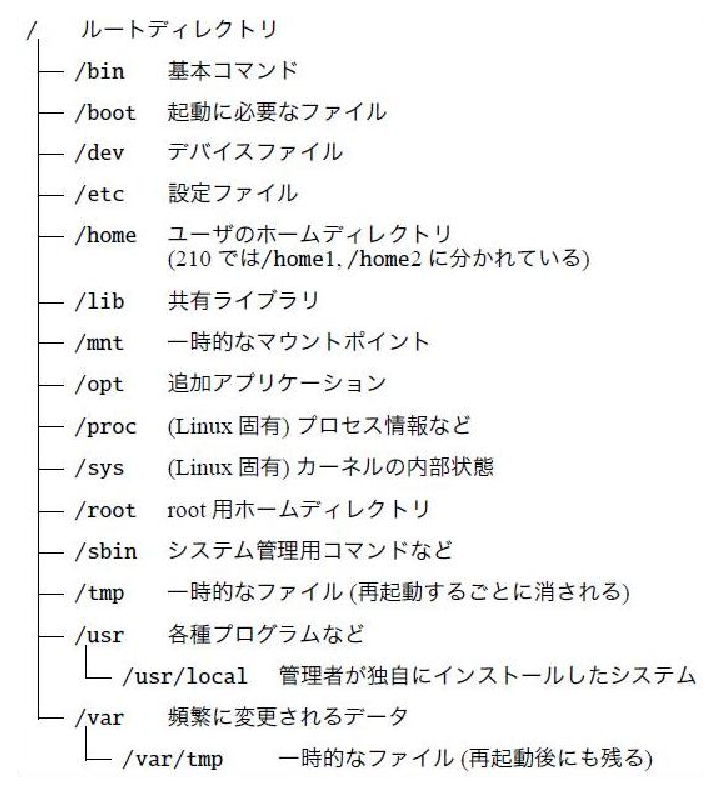
\includegraphics{images/fs-tree.eps}}
  \end{center}
  \caption{UNIX での代表的なディレクトリとその中身}
  \label{fig:fs-tree}
 \end{figure}

\begin{comment}

 \subsubsection{quota}
 UNIX では 1 台のマシンを複数のユーザが共有して使うことが多々あります。しかし
 ハードディスクの容量には限りがあるので、1 人のユーザが大量のデータをファイル
 に保存したりすると他のユーザがハードディスクを使えなくなってしまいます。

 それを解消するために、複数のユーザが共有するシステムでは quota と呼ばれる機
 構が働いていることがよくあります。これはユーザに対してディスクの使用量を制限
 するもので、ユーザ 1 人 1 人に対しもしくはグループ単位で、パーティション毎に
 ディスク使用量またはファイル数を制限することができます。
 \begin{description}
  \item[制限の方法]
   \begin{tabular}[t]{rl}
    \重要{block quota} & ディスクの割当を容量 (ブロック\footnotemark) で制限 \\
    \重要{inode quota} & ディスクの割当をファイル数 (inode 数) で制限 \\
                       & および、上記の組み合わせ
   \end{tabular}
   \footnotetext{ 通常は 1 block = 1 k byte = 1024 byte の単位で表示する。
     ファイルシステム上のブロックサイズとは限らない。}
  \item[\重要{ソフトリミット} (Soft Limit)] ~ \\
	     ソフトリミットとは、quota でディスクの使用量を制限されたユーザ
	     がそのパーティション上で使用可能な最大のディスク容量をいいます。
  \item[\重要{ハードリミット} (Hard Limit)] ~ \\
	     ハードリミットとは、ディスク使用量の絶対的な制限で、quota でディ
	     スクの使用量を制限されたユーザは、ハードリミットを越えることが
	     出来ません。
  \item[猶予期間 (Grace Time)] ~ \\
	     猶予期間とは、ソフトリミットが強制的に実行されるまでの期間のこ
	     とで、この期間にのみハードリミットまでディスクを使用することが
	     可能になります。通常は 1 週間程です。
 \end{description}
 つまり、ハードリミットはどうやっても超えることはできないのですが、ソフトリミッ
 トは超えられます。しかし{\gtfamily ソフトリミットを超えた状態で猶予期間を過ぎ
 るとログインができなくなります}。残念ながらsakuraではquotaが何故か入っていませんが、
 知識として知っておくと良いでしょう。


  \subsubsection{quota 関連のコマンド}
  自分の quota およびディスク使用量を知るには \command{quota} コマンド
  \footnote{ 210の端末ではquotaの設定をしていないので、コマンドを入力して
  もエラーとなります。eccsの端末では設定されているそうです。}を使用
  します。
  {\setlength\narrowframewidth{4em}
    \begin{terminal}%
~\$ quota -v
Disk quotas for user s222600 (uid 50600):
     Filesystem  blocks    quota    limit   grace   files   quota   limit   grace
     sakura:/home1    6852  9000000 10000000             325       0       0
     sakura:/home2      30   100000   100000             204       0       0\end{terminal}}
  のようにします。出力の \path{sakura:/home1} $\cdots$ の行は、\path{/home1} 以
  下のファイルシステムにおいて\footnote{ sakura というのは \path{/home1} が実際に
  存在しているマシンの名前です。}、現在のディスク使用量が 6852~kB であり、ソフ
  トリミットは 9000000~kB ($\approx$ 9~GB), ハードリミットは 10000000~kB
  ($\approx$ 10~GB) であることを示しています。また、所有するファイルの総数は
  325 個で、inode quota のソフトリミット・ハードリミットは共に 0, つまり無制限
  であることを表しています。
  もしも
  {\setlength\narrowframewidth{4em}
   \begin{terminal}%
~\$ quota -v
Disk quotas for user s12345 (uid 65432):
     Filesystem  blocks    quota   limit   grace   files   quota   limit   grace
     sakura:/home1 4733286* 4000000 5000000   4days   15290       0       0\end{terminal}}
  上記のような出力が得られた場合、使用しているディスク容量がソフトリミットを
  超えており、4 日以内に対処しなければログインできなくなることが示されていま
  す。
  
\end{comment}

\begin{comment}
  
\subsection{ユーザ・グループ(詳細)}
本編ではrootユーザの紹介のみでした。ここではもう少し詳細に取り扱います。
  
 \subsubsection{ユーザとグループ}
 ユーザには\重要{ユーザ名}と\重要{所属グループ}という情報があります。ユーザ名
 は説明するまでもなく、自分のユーザ名です。所属グループは自分の所属するグルー
 プであって、ユーザは少くとも一つのグループに所属し、複数のグループに所属する
 こともできます。ユーザの所属するグループのうち一つは特別なグループで\重要{プ
 ライマリグループ}と呼ばれ、ファイルなどを作成した時にそのファイルの所有グルー
 プとして使われます。

 グループへの所属登録自体は管理者 (root) が行います。また、ユーザ名やグループ
 名には数値で表された識別子 (ID) が関連付けられています。\command{id} コマンド
 を使うことで自分や他のユーザの情報を見ることができます。
 \begin{terminal}~\$ id\end{terminal}
 と打ってみて下さい。
 \begin{terminal}%
uid=50600(s222600) gid=20000(student) groups=20000(student)\end{terminal}
 のような出力
 が返ってきたと思います。

 これによって得られる表示のうち uid はユーザ ID とユーザ名、gid はプライマリグ
 ループ ID とプライマリグループ名、groups は自分の所属する全グループ ID とグ
 ループ名です。

 このように、演習室のマシンでは学生ユーザはみな student というグループに所属しています。
 admin210 のメンバーになるとこの他 admin (gid=21000) というグループにも所属する
 ようになります。また TA や教官は ta (gid=20090) というグループに所属していま
 す。また、
 \begin{terminal}~\$ id \argument{username}\end{terminal}
 でユーザ \argument{username} の情報をみることができます。

 \subsubsection{ファイルの所有者}
 UNIX ではそのファイルが誰のものかを
 \begin{enumerate}
  \item[1.] owner (所有者)
  \item[2.] group (所有グループ)
  \item[3.] other (他人)
 \end{enumerate}
 の 3 つに分けて区別しています。1. はそのファイルを所有する者、2. はそのファイ
 ルを所有するグループです。3. は所有者でなく 2. のグループにも属さないユーザを
 表わします。

 自分の所有するファイルでも owner を変更することはできませんが (root にはでき
 ます)、自分の所有するファイルなら自分の所属するグループのいずれかへファイルの
 グループを変更できます。このときに利用するコマンドは \command{chgrp} です。
 \begin{terminal}%
~\$ chgrp \argument{groupname} \argument{filename}
\end{terminal}
 これでファイル \argument{filename} の所有グループが \argument{groupname} に変
 更されます。ディレクトリの中身も全て所有グループを変えたいのならば
 「\term{-R}」オプションをつけます。
 \begin{terminal}%
~\$ chgrp -R \argument{groupname} \argument{dirname}
\end{terminal}
 但し、自分の所属しないグループを所有グループにすることはできませんので
 student グループにしか所属していない皆さんは \command{chgrp} コマンドを使うこ
 とはないでしょう。

\end{comment}
 


%\printindex

\end{document}


%%% Local Variables:
%%% mode: japanese-latex
%%% TeX-master: "01-shell"
%%% mode: auto-fill
%%% fill-column: 72
%%% End:
